\chapter{Swing-Up Design}\label{sec:swing-upDesign}
In this chapter three swing-up controllers are designed, all based on \cite{kjAastrom}. The pendulum is started at rest, $\theta = \pi$, with the angle convention specified in \autoref{fig:mechanicalDrawing}. The idea of the swing-up controller is to increase the mechanical energy in the system until it matches that of the desired end state, $\theta = 0$ and $\dot{\theta} = 0$, that is, the upright position at rest. The minimum energy in the system occurs at the starting position at rest, which is considered to be zero as mentioned in the \textit{Model} \autoref{sec:model}. So the target energy is $E_{\mathrm{eq}} = 2 m g l$, that is, the potential energy of the pendulum in the unstable equilibrium.

Consider the pendulum dynamics from \autoref{eq:energyDerivedDynamicEquation1}, where $J = m l^2$ is the pendulum inertia and frictions are assumed to be zero such that,
\begin{align}
  J \ddot{\theta} - m l \cos \theta a_c - m g l \sin \theta  &= 0 \ \ \ .  \label{eq:pendulumDynamics}
\end{align}
This equation captures the behavior of the pendulum corresponding to some controlled acceleration $a_c$ at the pivot point. This acceleration is viewed as the control input for now. The force needed to achieve this acceleration is considered at the end of the design. It is further convenient to describe the energy of the pendulum with the coordinate frame fixed at its pivot point, see \autoref{fig:fixedCooredinateSystem}.
%
\begin{figure}[H]
  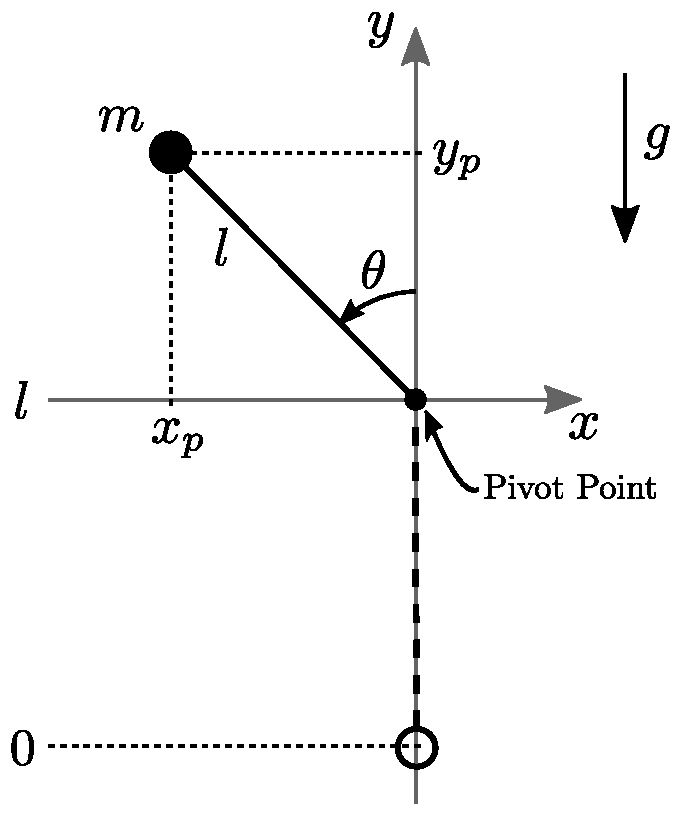
\includegraphics[width=.3\textwidth]{figures/fixedCooredinateSystem}
  \caption{The energy used in the swing-up controller is described using this convention, where the coordinate frame is fixed at the pivot point of the pendulum. The zero reference is placed as before s.t. all energies are positive.}
  \label{fig:fixedCooredinateSystem}
\end{figure}
%
From \autoref{fig:fixedCooredinateSystem}, the conversion from excessive to generalized coordinates is given by,
\begin{align}
  x_p  &= -l \sin \theta   \ \ \ ,\ \ \ y_p = l(\cos \theta + 1)  \ \ \ ,\ \ \ \dot{x}_p = -l \cos \theta \dot{\theta}  \ \ \ ,\ \ \ \dot{y}_p = -l \sin \theta \dot{\theta}  \ \ \ .  \label{eq:cooredinateConvertFixed}
\end{align}
The mechanical energy in this coordinate frame is then,
\begin{align}
  E_p &= m g y_p + \tfrac{1}{2} m \dot{x}_p^2 + \tfrac{1}{2} m \dot{y}_p^2   \label{eq:pendulumEnergy1} \\
  E_p &= m g l (\cos \theta +1) + \tfrac{1}{2} m (-l \cos \theta \dot{\theta})^2 + \tfrac{1}{2} m (-l \sin \theta \dot{\theta})^2  \label{eq:pendulumEnergy2} \\
  E_p &= m g l (\cos \theta +1) + \tfrac{1}{2} J (\cos^2 \theta  + \sin^2 \theta )\dot{\theta}^2   \label{eq:pendulumEnergy3} \\
  E_p &= \tfrac{1}{2} J \dot{\theta}^2 + m g l (\cos \theta +1) \ \ \ .   \label{eq:pendulumEnergy4}
\end{align}
The following sections explores different approaches of controlling the pendulum energy specified in \autoref{eq:pendulumEnergy4} to its desired reference.

\section{Energy Control}
A function candidate is proposed,
\begin{align}
  V(\theta, \dot{\theta}) &= \tfrac{1}{2} E_\Delta ^2 \ \ \ ,   \label{eq:lyapunovCandidate} 
\end{align}
where $E_\Delta$ is the difference in energy in relation to the unstable equilibrium,
%
\begin{align}
  E_\Delta &= E_p  - E_{\mathrm{eq}}   \label{eq:energyDelta1} \\
  E_\Delta &= \tfrac{1}{2} J \dot{\theta}^2 + m g l (\cos \theta +1) - 2 m g l  \label{eq:energyDelta2} \\
  E_\Delta &= \tfrac{1}{2} J \dot{\theta}^2 + m g l (\cos \theta -1)   \ \ \ ,  \label{eq:energyDelta3}
\end{align}
hence,
\begin{align}
  V &= \tfrac{1}{2}( \tfrac{1}{2} J \dot{\theta}^2 + m g l (\cos \theta -1)  ) ^2 \\ 
  V &= \tfrac{1}{2} (\tfrac{1}{2} J \dot{\theta}^2)^2 + \tfrac{1}{2} (m g l (\cos \theta -1)  ) ^2  +  \tfrac{1}{2} J \dot{\theta}^2  m g l (\cos \theta -1) \\
  V &= \tfrac{1}{8} J^2 \dot{\theta}^4 + \tfrac{1}{2} m^2 g^2 l^2 ( \cos^2 \theta + 1 -2\cos \theta )  +  \tfrac{1}{2} J \dot{\theta}^2  m g l (\cos \theta -1)  \ \ \ , \label{eq:lyapunovCandidate2}
\end{align}
further,
%\begin{align}
%  \frac{\partial^2 V}{\partial^2 \theta\dot{\theta}} &= -J \dot{\theta} m g l \sin \theta \ \ \ .  \label{eq:lyapunovCandidateDiff}
%\end{align}
\begin{align}
\frac{\partial V}{\partial \theta}       &= -m^2 g^2 l^2 \cos \theta \sin \theta + m^2 g^2 l^2 \sin \theta - \tfrac{1}{2} J \dot{\theta}^2 m g l \sin \theta \label{eq:lyapnovCandidateDiff_theta} \\
\frac{\partial V}{\partial \dot{\theta}} &=  \tfrac{1}{2} J^2 \dot{\theta}^3 + J m g l ( \cos \theta - 1 ) \dot{\theta} \ \ \ ,  \label{eq:lyapnovCandidateDiff_thetaDot}
\end{align}
where both \autoref{eq:lyapnovCandidateDiff_theta} and \ref{eq:lyapnovCandidateDiff_thetaDot} are continuous, $C^0$, so $V(\theta,\dot{\theta})$ is continuously differentiable, $C^1$, in the entire $\mathbb{R}^2$.

The idea is to reach the reference $E_\Delta = 0$, which happens when,
\begin{align}
  \tfrac{1}{2} J &\dot{\theta}^2 + m g l (\cos \theta -1) = 0 \label{eq:energyDeltaZero1} \\
  &\dot{\theta} = \pm \left(\frac{-2 m g l (\cos \theta -1)}{J}\right)^{\tfrac{1}{2}}  \ \ \ .  \label{eq:energyDeltaZero2}
\end{align}
%
A plot of \autoref{eq:energyDeltaZero2} in the phase plane, see \autoref{fig:orbit}, reveals a set of solutions joining the two unstable equilibrium points.
%
\begin{figure}[H]
  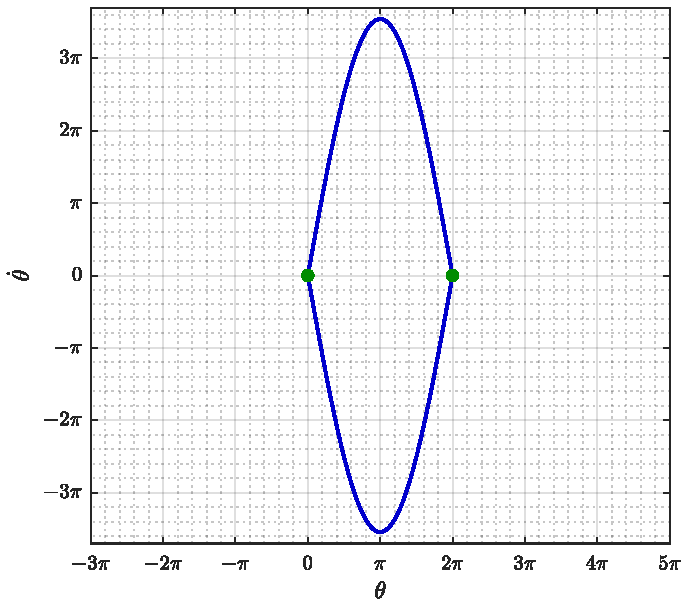
\includegraphics[width=.4\textwidth]{figures/orbit}
  \caption{If the trajectories of the system are restricted to this set, the energy error is maintained at zero and the trajectories form a heteroclinic orbit.}
  \label{fig:orbit}
\end{figure}
%
If the energy reference is successfully tracked, the system will be restricted to this set rather than a single equilibrium point. Such a trajectory joining two equilibrium points is called a heteroclinic orbit.\\
Recall the system from \autoref{eq:pendulumDynamics},
\begin{align}
  J \ddot{\theta} &= m l \cos \theta a_c + m g l \sin \theta \ \ \ ,  \label{eq:pendulumDynamics2}
\end{align}
the derivative of $V$ is then evaluated along trajectories of the system,
\begin{align}
  \dot{V} &= E_\Delta \dot{E}_\Delta % \ \ \ ,\ \ \ \ \dot{E}_\Delta = J \dot{\theta} \ddot{\theta} - m g l \sin \theta \dot{\theta}
  \label{eq:lyapunovDerivative1} \\ 
  \dot{V} &= E_\Delta ( J \dot{\theta} \ddot{\theta} - m g l \sin \theta \dot{\theta} )   \label{eq:lyapunovDerivative2} \\
  \dot{V} &= E_\Delta ( \dot{\theta} ( m l \cos \theta a_c + m g l \sin \theta )  - m g l \sin \theta \dot{\theta} )   \label{eq:lyapunovDerivative3} \\
  \dot{V} &= m l E_\Delta \cos \theta \dot{\theta} a_c   \ \ \ .  \label{eq:lyapunovDerivative4}
\end{align}
The idea is to find a control law, $a_c$, which allows trajectories of the system to reach the desired heteroclinic orbit.
%is $C^0$ and thus $V(x)$ is continuously differentiable, $C^1$. Further, $V(\vec{0}) = 0$ and $V(\vec{x})>0$ in the entire state space, excluding zero.
%
%The Lyapunov function candidate, \autoref{eq:lyapunovCandidate}, is continuously differentiable in the entire $\mathbb{R} ^2$. Its derivative is evaluated to find a stabilizing controller,
%
%\begin{theorem}[Lyapunov Stability Theorem]
%  \label{th:lyapunovStabilityTheorem}
%  Consider the autonomous system, $f(\vec{x}) = \dot{\vec{x}}$, where $f : \mathbb{D} \rightarrow \mathbb{R} ^n$ is locally Lipschitz and $\vec{x}=\vec{0}$ is an equilibrium point. Then if $\exists\ V : \mathbb{D} \rightarrow \mathbb{R}$ and \vspace{-12pt}
%  \begin{enumerate}
%    \item $V(\vec{x})$ is $C^1$
%    \item $V(\vec{x}) > 0$ $\forall \vec{x} \in \mathbb{D}\backslash 0$ and $V(\vec{0}) = 0$
%    \item $\dot{V}(\vec{x}) \leq 0$ in $\mathbb{D}$
%  \end{enumerate} \vspace{-12pt}
%  then $\vec{x} = \vec{0}$ is stable. Further, if,
%  \vspace{-12pt}
%  \begin{itemize}
%    \item[] $ \dot{V}(\vec{x}) < 0\ \mathrm{in}\ \mathbb{D}\backslash 0  \ \ \ ,  $
%  \end{itemize}\vspace{-12pt}
%  then $\vec{x} = \vec{0}$ is asymptotically stable \cite{HKKhalil}.
%\end{theorem}\vspace{-12pt}
%
%The third condition states that the derivative of the Lyapunov function candidate along trajectories of the system must be less than or equal to zero in the entire state space. In this case, from \autoref{eq:lyapunovDerivative1}, if the energy error goes to zero, so does the derivative of the Lyapunov function.\\
%Without checking for definiteness, it is known that in cases where $V(\vec{x}) = 0$, trajectories neither approach nor diverge from the equilibrium, but rather stay in some orbit. While \autoref{th:lyapunovStabilityTheorem} has the potential to promise stability of the desired orbit once there, it does not guarantee convergence to said orbit.\\
By studying LaSalle's \autoref{th:lasallesTheorem}, analysis of convergence to sets is made possible.

\begin{minipage}[]{\linewidth}
  \begin{theorem}[LaSalle's Theorem]
    \label{th:lasallesTheorem}
    %Consider again the system from \autoref{th:lyapunovStabilityTheorem}.
    Consider the autonomous system, $f(\vec{x}) = \dot{\vec{x}}$, where $f : \mathbb{D} \rightarrow \mathbb{R} ^n$ is locally Lipschitz and $\vec{x}=\vec{0}$ is an equilibrium point. Then if there exist some function $V : \mathbb{D} \rightarrow \mathbb{R}$ and
    \begin{enumerate}
      \item $V(\vec{x})$ is $C^1$
      \item $\exists\ c > 0$ s.t. $\Omega_c = \{\vec{x} \in \mathbb{R}^n \ | \ V(\vec{x}) \leq c \} \subset \mathbb{D}$ is bounded
      \item $\dot{V}(\vec{x}) \leq 0 \ \ \forall \ \vec{x} \in \Omega_c$
    \end{enumerate}
    then $\vec{x}(0) \in \Omega_c \Rightarrow \vec{x}(t) \xrightarrow[]{t \to \infty} M \ ,$  where $M$ is the largest invariant set in
    \begin{itemize}
      \item[] $E = \{ \vec{x} \in \Omega_c \ | \ \dot{V}(\vec{x}) = 0 \} \ \ $ \cite{HKKhalil}.
    \end{itemize}
  \end{theorem}
\end{minipage}
%
%Further, $V(\vec{0}) = 0$ and $V(\theta, \dot{\theta})>0$ in the domain $ [\ 0 ; 2\pi \ )$.
The first condition in LaSalle's \autoref{th:lasallesTheorem} is already satisfied. Notice that the function candidate, $V(\vec{x})$, is not required to be positive definite.\\
The second condition states that some bounded set, $\Omega_c$, of solutions for which $V(\vec{x})$ is less than or equal to some constant $c$ must exist.\\
This ties into the third condition stating that the derivative of the function candidate must be negative semi-definite along trajectories of the system for all solutions in said set.\\
%To find $\Omega_c$, the derivative of the function candidate,  \autoref{eq:lyapunovDerivative1}, is evaluated along the trajectories of the system, \autoref{eq:pendulumDynamics},
%\begin{align}
%  \dot{V} &= E_\Delta ( J \dot{\theta} \ddot{\theta} - m g l \sin \theta \dot{\theta} )   \label{eq:lyapunovDerivative2} \\
%  \dot{V} &= E_\Delta ( \dot{\theta} ( m l \cos \theta a_c + m g l \sin \theta )  - m g l \sin \theta \dot{\theta} )   \label{eq:lyapunovDerivative3} \\
%  \dot{V} &= m l E_\Delta \cos \theta \dot{\theta} a_c   \ \ \ ,  \label{eq:lyapunovDerivative4}
%\end{align}
%
The controlled acceleration at the pivot point, $a_c$, is then designed to satisfy the third condition in \autoref{th:lasallesTheorem},
\begin{align}
  a_c &= -k E_\Delta \cos \theta \dot{\theta}  \ \ \ ,  \label{eq:accControlLaw}
\end{align}
where the tuning parameter, $k>0$, is introduced to allow scaling the control output to fit the capabilities of the actuator. Inserting the control law yields,
\begin{align}
  \dot{V} &= m l E_\Delta \cos \theta \dot{\theta} a_c  \\
  \dot{V} &= m l E_\Delta \cos \theta \dot{\theta} (-k E_\Delta \cos \theta \dot{\theta})     \label{eq:lyapunovDerivativeControlled1} \\
  \dot{V} &= -k m l (E_\Delta \cos \theta \dot{\theta})^2  \leq 0  \ \ \ ,   \label{eq:lyapunovDerivativeControlled2} 
\end{align}
satisfying the third condition of \autoref{th:lasallesTheorem} not only in $\Omega_c$ but in the entire state space. This means any $\infty>c>0$ will satisfy the second condition. However, looking at the function candidate,
\begin{align}
V &= \tfrac{1}{8} J^2 \dot{\theta}^4 + \tfrac{1}{2} m^2 g^2 l^2 ( \cos^2 \theta + 1 -2\cos \theta )  +  \tfrac{1}{2} J \dot{\theta}^2  m g l (\cos \theta -1)  \ \ \ , \label{eq:functionCandidate3}
\end{align}
the angle is only present in periodic functions. Hence no value of $c$ can bound the angle. If starting some arbitrary place in the state space, the energy reference is eventually tracked, but the heteroclinic orbit could settle between any two saddle points. To constrain further analysis and design to the desired region of operation, $\Omega_c$ is defined as the set containing all points within and on the set in \autoref{fig:orbit}, that is,
\begin{align}
  \Omega_c &=  \{ \vec{x} \ | \ \dot{\theta} \leq \left(\frac{-2 m g l (\cos \theta -1)}{J}\right)^{\tfrac{1}{2}} , \ 0 \leq \theta \leq 2 \pi  \} \ \ \ . \label{eq:omegaC}
\end{align}
%
%It also satisfies the first stability criterion of \autoref{th:lyapunovStabilityTheorem}, indicating the control law has caused stability of the previously unstable equilibrium. However, the stability is not asymptotical and $\vec{x} = \vec{0}$ is not the only stable point when using this control strategy. Further, as stated, \autoref{th:lyapunovStabilityTheorem} does not guarantee convergence to a set.\\
All conditions of LaSalle's \autoref{th:lasallesTheorem} are satisfied, thus, if starting in $\Omega_c$, trajectories of the system will converge to $M$ as time goes to infinity. $M$ is the largest invariant set in $E$, which can be described as the union of sets for which \autoref{eq:lyapunovDerivativeControlled2} is zero,
\begin{align}
  A &=  \{ \vec{x} \in \Omega_c \ | \ E_\Delta     = 0 \}      \\
  B &=  \{ \vec{x} \in \Omega_c \ | \ \cos \theta  = 0 \}  \\
  C &=  \{ \vec{x} \in \Omega_c \ | \ \dot{\theta} = 0 \}  \\
  E &= A \cup B \cup C \ \ \ . \label{eq:E}
\end{align}
To construct set $M$ it is necessary to evaluate each set for invariance with respect to the controlled system. A proof is developed to show invariance of the first set.
\begin{proof}[Invariance of Set A]
  \label{pr:invariantA}
  Recall the relation between $\dot{\theta}$ and $\theta$ for $E_\Delta = 0$,
  \begin{align}
    &\dot{\theta}_z = \pm \left(\frac{-2 m g l (\cos \theta -1)}{J}\right)^{\tfrac{1}{2}}  \ \ \ ,  \label{eq:thetaDotForEDeltaZero}
  \end{align}
  where $\dot{\theta}_z$ is the angular velocity for which the energy error is zero. Further, consider the model in following form,
  \begin{align}
    \ddot{\theta} &= \tfrac{1}{J} ( m l \cos \theta a_c + m g l \sin \theta ) \ \ \ .  \label{eq:pendulumDynamics3}
  \end{align}
  To prove that $A$ is invariant with respect to \autoref{eq:pendulumDynamics3}, the slope of $\dot{\theta}_z$ is compared to the slope of the controlled system trajectories in the set. If the slopes are equal, then no trajectory can leave the set $A$, thus proving $A$ is invariant with respect to the controlled system. The slope of $\dot{\theta}_z$ is,
  \begin{align}
    \frac{\partial \dot{\theta}_z}{\partial \theta} &= \pm \frac{m g l \sin\theta}{ J } \left(\frac{-2 m g l (\cos \theta -1)}{J}\right)^{-\tfrac{1}{2}} \\
    \frac{\partial \dot{\theta}_z}{\partial \theta} &= \frac{m g l \sin\theta}{ J \rule{0pt}{12pt}\dot{\theta}_z}  \ \ \ .  \label{eq:thetaDotForEDeltaZero_dTheta}
  \end{align}
  The slope of the trajectories of the controlled system, \autoref{eq:pendulumDynamics3}, in set $A$ is then,
  \begin{align}
    b &= \frac{\ddot{\theta}_z}{\rule{0pt}{12pt}\dot{\theta}_z} \\
    b &= \frac{- m l \cos \theta a_c( \theta, \dot{\theta}_z ) + m g l \sin \theta}{ J \rule{0pt}{12pt}\dot{\theta}_z} \\
    b &= \frac{- k m l \cos^2 \theta E_\Delta( \theta, \dot{\theta}_z ) \dot{\theta}_z + m g l \sin \theta}{ J \rule{0pt}{12pt}\dot{\theta}_z} \\
    b &= \frac{- k m l \cos^2 \theta ( \tfrac{1}{2} J \dot{\theta}_z^2 + m g l (\cos \theta -1)  ) \dot{\theta}_z}{ J \rule{0pt}{12pt}\dot{\theta}_z}  +  \frac{m g l \sin \theta}{ J \rule{0pt}{12pt}\dot{\theta}_z} \\
    b &= - k m l \cos^2 \theta \tfrac{1}{2} \dot{\theta}_z^2 - \tfrac{1}{J} k m l \cos^2 \theta m g l (\cos \theta -1)  +  \frac{m g l \sin \theta}{ J \rule{0pt}{12pt}\dot{\theta}_z} \\
    %b &= - k m l \cos^2 \theta \tfrac{1}{2} \left( \pm \left(\frac{-2 m g l (\cos \theta -1)}{J}\right)^{\tfrac{1}{2}} \right)^2 \\
    %  &- \tfrac{1}{l^2 m} k m^2 l^2 g \cos^2 \theta (\cos \theta -1)  +  \frac{m g l \sin \theta}{ J \rule{0pt}{12pt}\dot{\theta}_z} \\
    b &= - k m l \cos^2 \theta \tfrac{1}{2} \left(\frac{-2 m g l (\cos \theta -1)}{J}\right)  - \tfrac{1}{l^2 m} k m^2 l^2 g \cos^2 \theta (\cos \theta -1)  +  \frac{m g l \sin \theta}{ J \rule{0pt}{12pt}\dot{\theta}_z} \\
    b &= - k m l \cos^2 \theta \tfrac{1}{2} \frac{-2 m g l (\cos \theta -1)}{l^2 m} - k \cos^2 \theta m g (\cos \theta -1)  +  \frac{m g l \sin \theta}{ J \rule{0pt}{12pt}\dot{\theta}_z}  \\
    b &= k \cos^2 \theta m g (\cos \theta -1) - k \cos^2 \theta m g (\cos \theta -1)  +  \frac{m g l \sin \theta}{ J \rule{0pt}{12pt}\dot{\theta}_z} \\
    b &= \frac{m g l \sin \theta}{ J \rule{0pt}{12pt}\dot{\theta}_z} \ \ \ ,  \label{eq:systemTrajSlopeInSetA}
  \end{align}
  where $\ddot{\theta}_z$ is the angular acceleration of the controlled system in set $A$.\\
  Finally, since,
  \begin{align}
    \frac{\partial \dot{\theta}_z}{\partial \theta} &= b \ \ \ ,  \label{eq:slopesEqual}
  \end{align}
  the set $A$ is invariant with respect to the controlled system.\vspace{-4pt}
  \begin{align}
    \tag*{$\blacksquare\ $}
  \end{align}
\end{proof}
%
\vspace{-8pt}
The set $B$ is invariant only for the intersection $B \cap A$, any other values of the angular velocity will cause it to leave the set since $\cos \theta = 0$ corresponds to a horizontal position of the pendulum. A similar argument can be made for set $C$, however, in this case if $\theta = \pi$, the system stays in the set. So, the invariant part of set $C$ excluding $A$ is,
\begin{align}
  F &=  \{ \vec{x} \in \Omega_c \ | \ \dot{\theta} = 0 \ , \ \theta = \pi \}  \ \ \ ,  \label{eq:F}
\end{align}
thus the largest invariant set in $E$ is,
\begin{align}
M &= A \cup F \ \ \ .  \label{eq:M}
\end{align}
%
The sets are visualized in \autoref{fig:setPlot}.
\begin{figure}[H]
  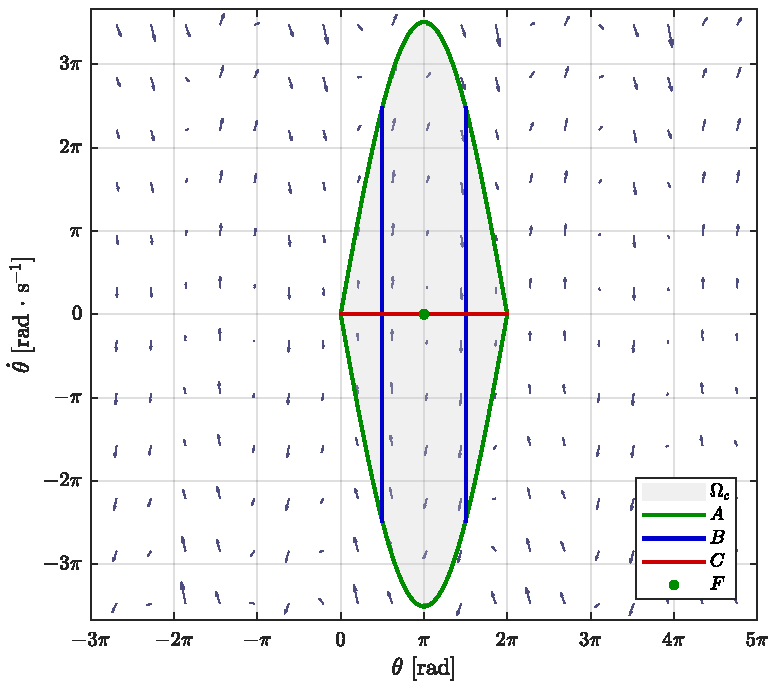
\includegraphics[width=.65\textwidth]{figures/setPlot}
  \caption{The set $\Omega_c$ shown along with sets in $\Omega_c$ for which $\dot{V}(\vec{x}) = 0$. Set $A$ and $F$ together form the largest invariant set $M$ in $E$. The phase portrait of the controlled system shows how its trajectories line up with $A$ as stated by \autoref{pr:invariantA}.}
  \label{fig:setPlot}
\end{figure}
%
If this control law is started at zero angular velocity, $\dot{\theta} = 0$, in the stable equilibrium, the computed control is maintained at zero and the pendulum never swings up. So for this control law to work, the pendulum must be started slightly away from the stable equilibrium.

An extra step is needed to apply this control strategy. So far the control output is an acceleration, $a_c$, at the pivot point. It is possible to input the desired acceleration, $a_c$, into the second dynamic equation, \autoref{eq:energyDerivedDynamicEquation1}, and solve for the force needed to achieve this acceleration,
%
\begin{align}
  u &=  ( M + m )a_c + m l \sin x_1 x_3^2 - m l \cos x_1 \dot{x}_3  \ \ \ ,
  \label{eq:forceDynamics}
\end{align}
%
where the cart friction coefficients are set to zero again.\\
To calculate the force from this expression, \autoref{eq:forceDynamics}, it is also necessary to know the angular acceleration of the pendulum, $\dot{x}_3$, which can be solved for in the system dynamics, \autoref{eq:nonlinearStateSpace}, inserting known states and control input applied in the previous step,
%
\begingroup\makeatletter\def\f@size{10}\check@mathfonts
\def\maketag@@@#1{\hbox{\m@th\normalsize\normalfont#1}}%
\begin{align}
  \begin{bmatrix}
    \dot{x}_3  \\
    \dot{x}_4
  \end{bmatrix}
  &=
  \begin{bmatrix}
    m l^2           & -m l \cos x_1  \\
    -m l \cos x_1   & M + m
  \end{bmatrix}^{-1}
  \begin{bmatrix}
    - b_{p,v} x_3 - \tanh(\text{k}_\text{tanh}x_3) b_{p,c} + m g l \sin x_1 \\
    u_{last} - m l \sin x_1 x_3^2
  \end{bmatrix}
  \ \ \ ,
  \label{eq:nonlinearStateSpaceQdotDot} \\ \nonumber
\end{align}
\endgroup \vspace{-44pt}

%
where $u_{last}$ is the force applied in the previous step.\\
From \autoref{eq:nonlinearStateSpaceQdotDot} the approximated angular acceleration is then,
\begingroup\makeatletter\def\f@size{10}\check@mathfonts
\def\maketag@@@#1{\hbox{\m@th\normalsize\normalfont#1}}%
\begin{align}
\dot{x}_3 &= \frac{ ( M + m )(- b_{p,v} x_3 - \tanh(\text{k}_\text{tanh}x_3) b_{p,c} + m g l \sin x_1) }{ l^2 m ( M + m - m \cos^2 x_1 ) } + \frac{ \cos x_1 (u_{last} - m l \sin x_1 x_3^2) }{ l ( M + m - m \cos^2 x_1 ) }
\ \ \ .
\label{eq:thetaDotDotApprox} \\ \nonumber
\end{align}
\endgroup \vspace{-44pt}

%
Inserting \autoref{eq:thetaDotDotApprox} into \autoref{eq:forceDynamics} results in the control input, $u$, necessary to achieve the desired acceleration, $a_c$, at the pivot point. This method is used for all three swing-up controllers, so to avoid excessive notation the proceeding energy control laws are derived with $a_c$ as the control parameter.

All simulations are performed using the nonlinear state space representation in \autoref{eq:nonlinearStateSpace} and the matlab ODE45 solver with a relative tolerance of \SI{1e-7}{}. Initializing the angle, $\theta$, at $\pi-0.1$ to avoid zero control output as discussed, the energy difference struggles to reach its reference at zero, see \autoref{fig:Edelta_1_noConX}. The pendulum friction and cart inertia are included in the calculation of the force needed to obtain the desired acceleration. This, however, is not concerned with what is needed to obtain the required energy. So the offset seen in \autoref{fig:Edelta_1_noConX} is caused by the control law, \autoref{eq:accControlLaw}, asking for insufficient acceleration.
%
\begin{figure}[H]
  \hspace{-10pt}
  \captionbox
  {
    Simulation of the first energy control method. The energy error struggles to maintain zero value, due to pendulum friction and cart inertia exchanging energy with the pendulum.
    \label{fig:Edelta_1_noConX}
  }
  {
    \hspace{-1cm}
    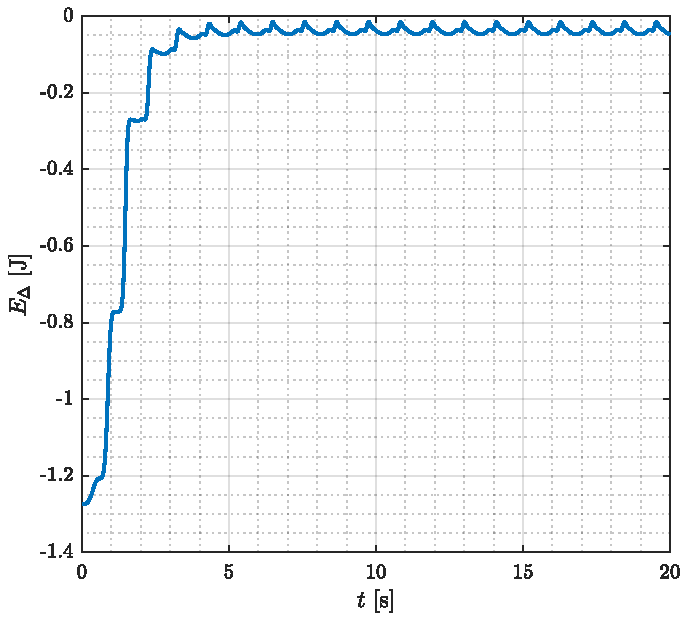
\includegraphics[width=.455\textwidth]{figures/Edelta_1_noConX}
  }
  \hspace{20pt}
  \captionbox 
  {
    This phase portrait shows the attempt to reach the heteroclinic orbit. It falls short due to the insufficient acceleration asked by the control law.
    \label{fig:phase_1_noConX}
  }
  {
    \hspace{-1cm}
    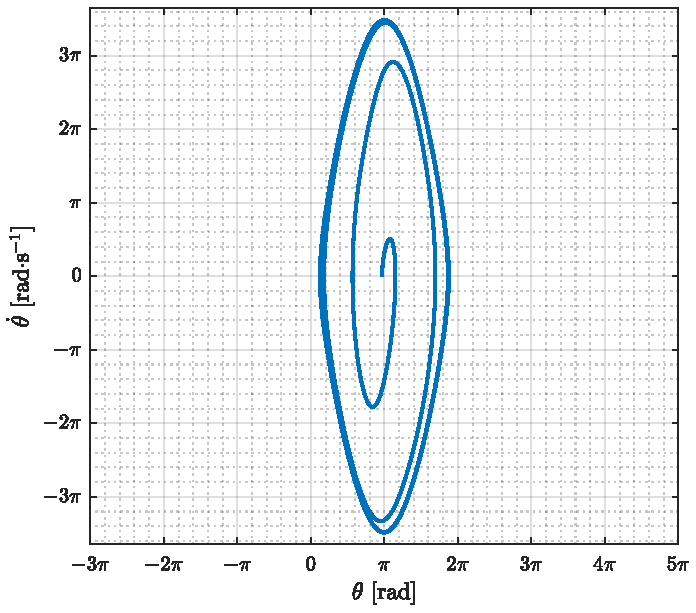
\includegraphics[width=.46\textwidth]{figures/phase_1_noConX}
  }  
\end{figure}
%
The pendulum also falls short of reaching the heteroclinic orbit, see \autoref{fig:phase_1_noConX}.
Further, since the energy of the pendulum is not affected by the position or velocity of the cart, this control law, \autoref{eq:accControlLaw}, is not concerned with controlling these. This becomes a problem in the physical setup as it has a rail length of \SI{0.89}{m}, see \autoref{table:systemParameters}. A traced animation is used to demonstrate this problem in \autoref{fig:ani_1_noConX}.
\begin{figure}[H]
  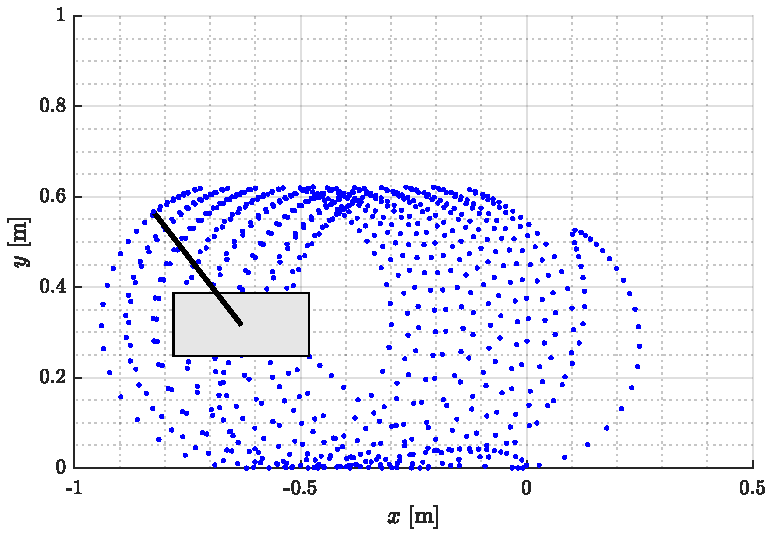
\includegraphics[width=.7\textwidth]{figures/ani_1_noConX}
  \caption{The cart drifts beyond the bounds of the physical system. This might not be a problem if the catch controller catches the pendulum in first try, but there is no guarantee of this being the case.}
  \label{fig:ani_1_noConX}
\end{figure}
%
An other issue is the actuation which is limited in the real system by the maximum allowed continuous current, see \autoref{table:systemParameters}. By tuning the parameter $k$ in the control law, better performance can be obtained, however at the cost of excessive actuation.
%
\begin{figure}[H]
  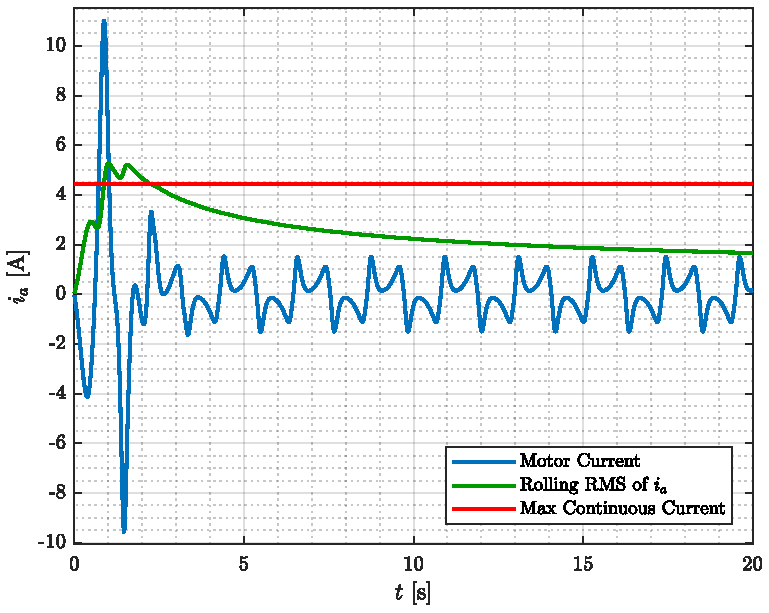
\includegraphics[width=.52\textwidth]{figures/ia_1_noConX}
  \caption{The motor current has high peaks in the beginning which likely exceeds the capabilities of the motor. The controller is tuned such that the RMS value of the current does not exceed the maximum continuous current requirement of the motor for a sustained period of time.}
  \label{fig:ia_1_noConX}
\end{figure}
%
For these graphs $k=1.3$ to keep the motor current at acceptable levels. The motor current is shown in \autoref{fig:ia_1_noConX} where the rolling RMS of $i_a$ is used to approximate the continuous current load on the motor. Though the continuous current is acceptable, the peaks in the start will be saturated in the real system, which would cause a longer rise time for the energy.

%\begin{figure}[H]
%  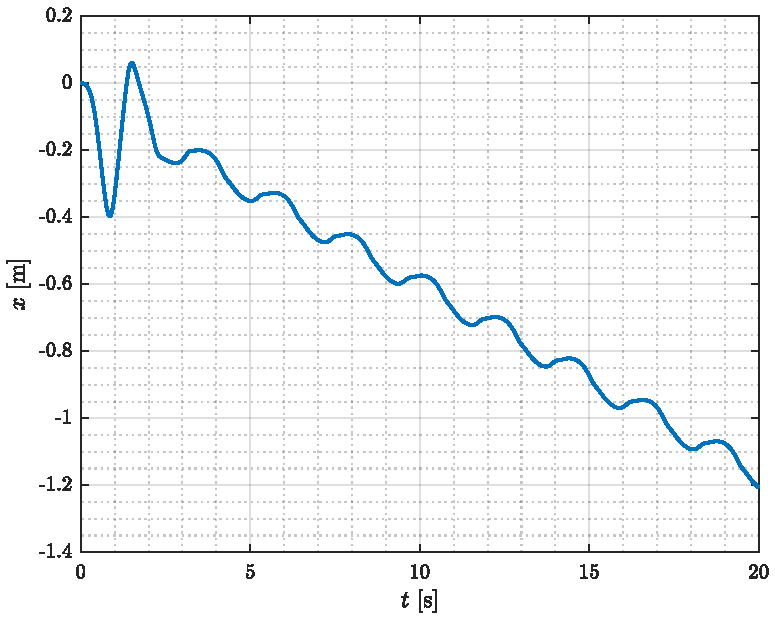
\includegraphics[width=.6\textwidth]{figures/x_1_noConX}
%  \caption{x1noConX}
%  \label{fig:x_1_noConX}
%\end{figure}
%\begin{figure}[H]
%  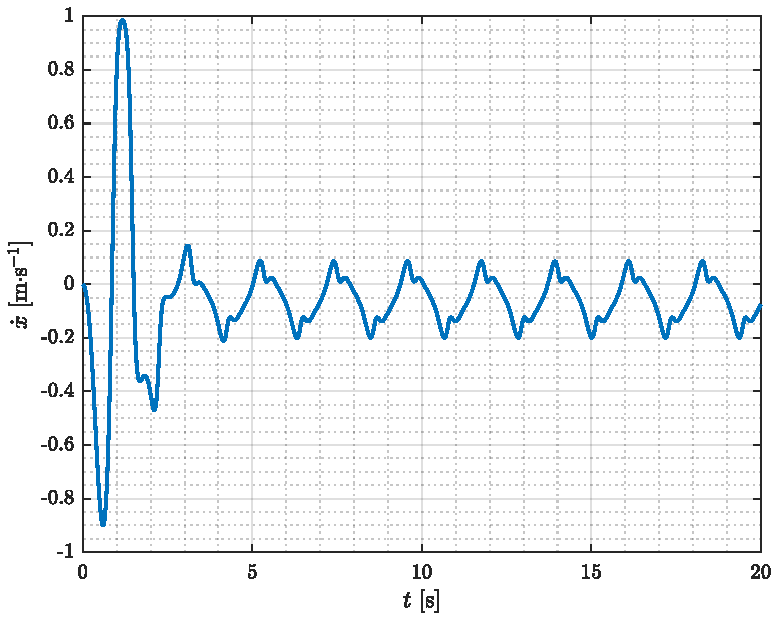
\includegraphics[width=.6\textwidth]{figures/xDot_1_noConX}
%  \caption{xDot1noConX}
%  \label{fig:xDot_1_noConX}
%\end{figure}
%\begin{figure}[H]
%  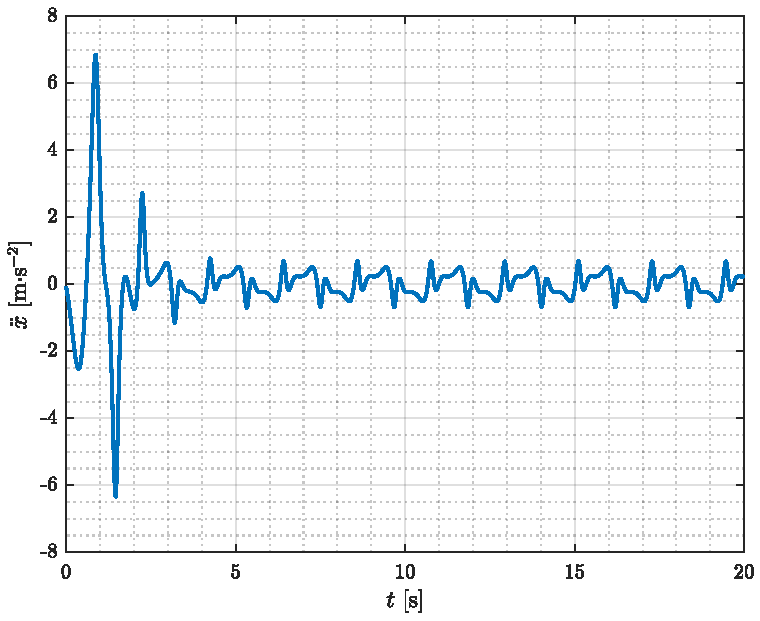
\includegraphics[width=.6\textwidth]{figures/xDotDot_1_noConX}
%  \caption{xDotDot1noConX}
%  \label{fig:xDotDot_1_noConX}
%\end{figure}
%\begin{figure}[H]
%  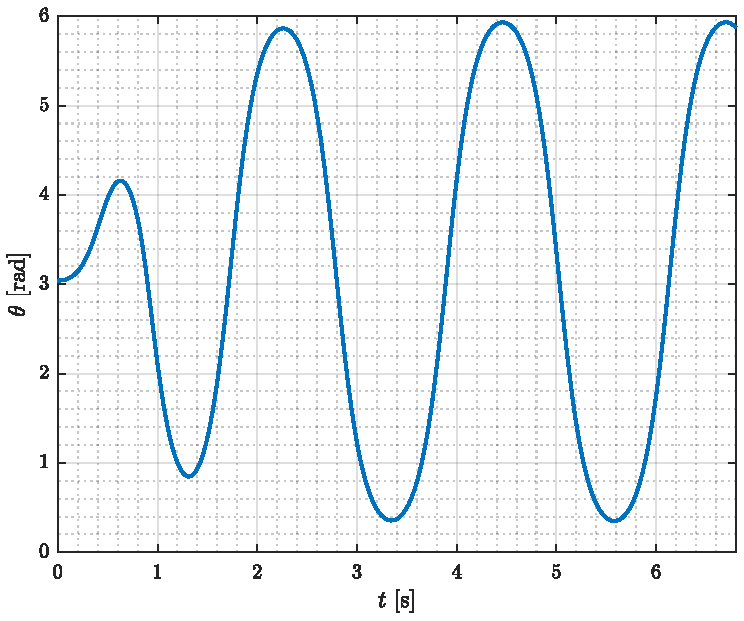
\includegraphics[width=.6\textwidth]{figures/theta_1_noConX}
%  \caption{theta1noConX}
%  \label{fig:theta_1_noConX}
%\end{figure}
%\begin{figure}[H]
%  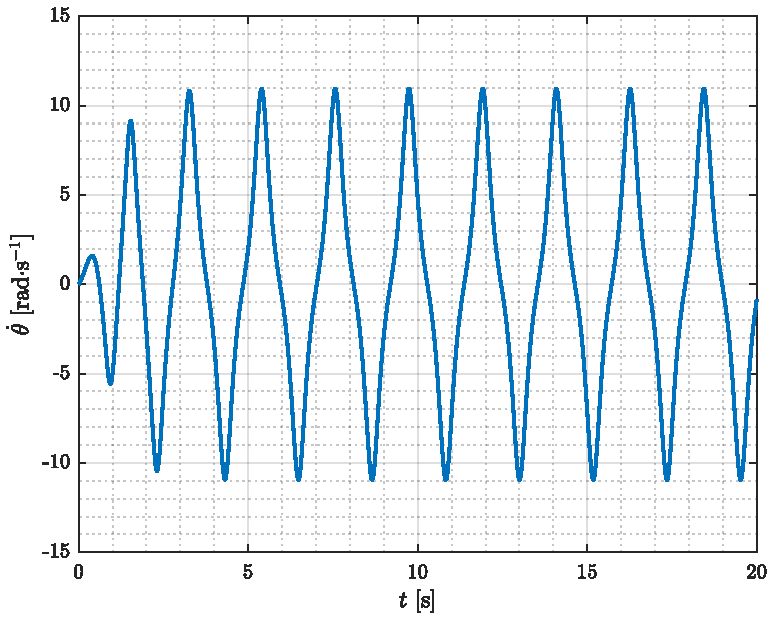
\includegraphics[width=.6\textwidth]{figures/thetaDot_1_noConX}
%  \caption{thetaDot1noConX}
%  \label{fig:thetaDot_1_noConX}
%\end{figure}
%\begin{figure}[H]
%  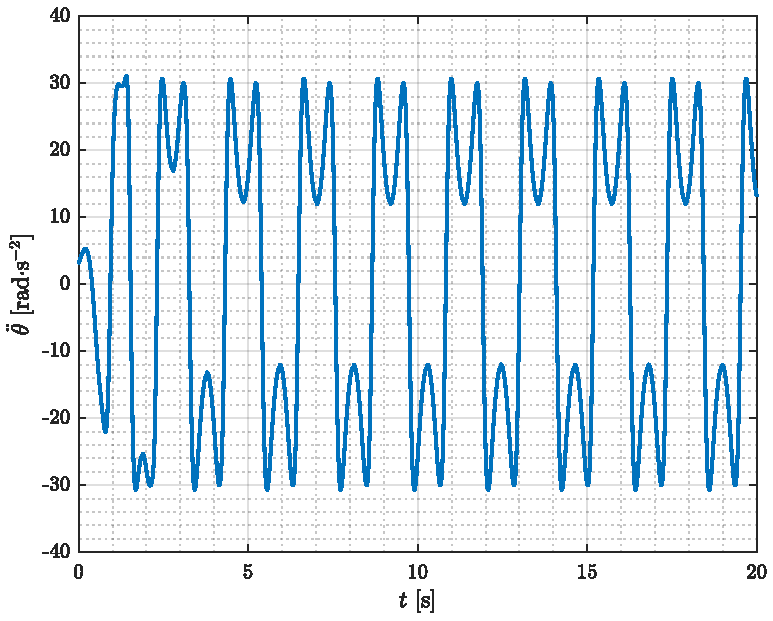
\includegraphics[width=.6\textwidth]{figures/thetaDotDot_1_noConX}
%  \caption{thetaDotDot1noConX}
%  \label{fig:thetaDotDot_1_noConX}
%\end{figure}


\section{Sign-Based Energy Control}
There are other ways to satisfy \autoref{eq:lyapunovDerivativeControlled2} than the control law suggested in \autoref{eq:accControlLaw}. To achieve maximal actuation a sign-function can be used to determine the direction of actuation along with a gain $k$ to adjust for the limits of the actuator as before,
\begin{align}
  a_c &= k\ \mathrm{sgn}(-E_\Delta \cos \theta \dot{\theta})  \ \ \ ,  \label{eq:accControlLaw2} 
\end{align}
where,
\begin{align}
\text{sgn}( s(\theta,\dot{\theta}) ) &=
\begin{cases}
\ \ \phantom{-} 1  & \ \ s  > 0 \ \lor   \ \cos \theta \dot{\theta} \ =    0 \\
\ \ \phantom{-} 0  & \ \ s  = 0 \ \land  \ \cos \theta \dot{\theta} \ \neq 0 \\
\ \            -1  & \ \ s  < 0 \hspace{3cm} ,
\end{cases}
\label{eq:sgnFunction}
\end{align}
to avoid no actuation when starting at stable equilibrium. This adjustment reduces the set,
\begin{align}
  M  &= \{ \vec{x} \in \Omega_c \ | \ E_\Delta = 0 \}  \ \ \ ,  \label{eq:M2}
\end{align}
such that convergence to $M$ when starting in $\Omega_c$, by \autoref{th:lasallesTheorem}, now assures convergence to the energy reference and thus to the heteroclinic orbit.\\
The gain is tuned to $k = 2.7$ in the following simulation. Looking at the energy in \autoref{fig:Edelta_2_noConX}, this strategy seems to work really well. From the phase portrait in \autoref{fig:phase_2_noConX} it is evident that a near perfect heteroclinic orbit is reached.
\begin{figure}[H]
  \hspace{-10pt}
  \captionbox
  {
    Using maximum actuation in the appropriate direction drives the energy error to zero and keeps it there.
    \label{fig:Edelta_2_noConX}
  }
  {
    \hspace{-1cm}
    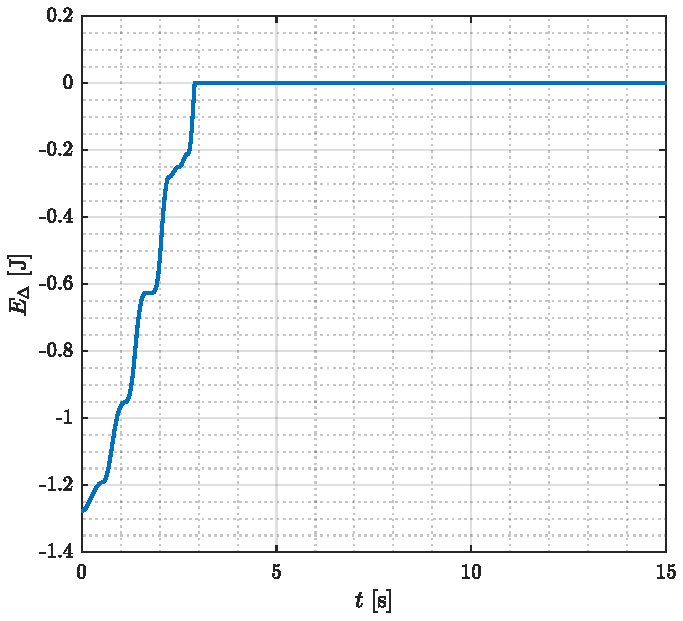
\includegraphics[width=.453\textwidth]{figures/Edelta_2_noConX}
  }
  \hspace{20pt}
  \captionbox 
  {
    The heteroclinic orbit is reached very accurately.
    \label{fig:phase_2_noConX}
  }
  {
    \hspace{-1cm}
    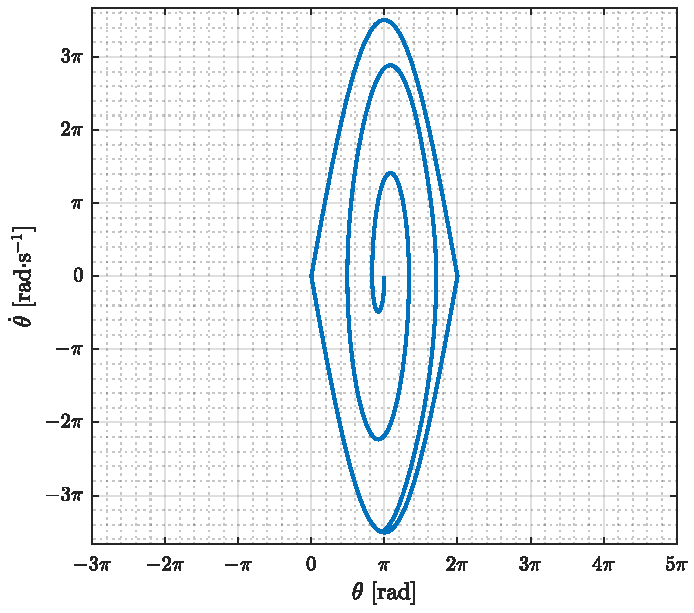
\includegraphics[width=.46\textwidth]{figures/phase_2_noConX}
  }  
\end{figure}
%
In \autoref{fig:ani_2_noConX} however, while the angle reaches the equilibrium as closely as possible without overshooting, this control law, as with the previous, does not account for position of the cart.
%
\begin{figure}[H]
  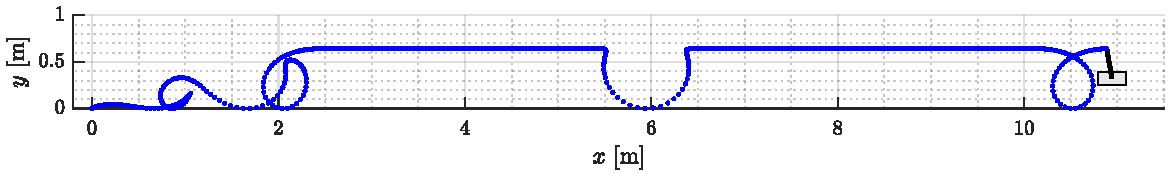
\includegraphics[width=1\textwidth]{figures/ani_2_noConX}
  \caption{The cart drifts as before, since the controller is only concerned with the energy of the pendulum.}
  \label{fig:ani_2_noConX}
\end{figure}
%
However, the bigger problem with this control law is obvious from \autoref{fig:ia_2_noConX}, where excessive switching shows on the control output.
%
\begin{figure}[H]
  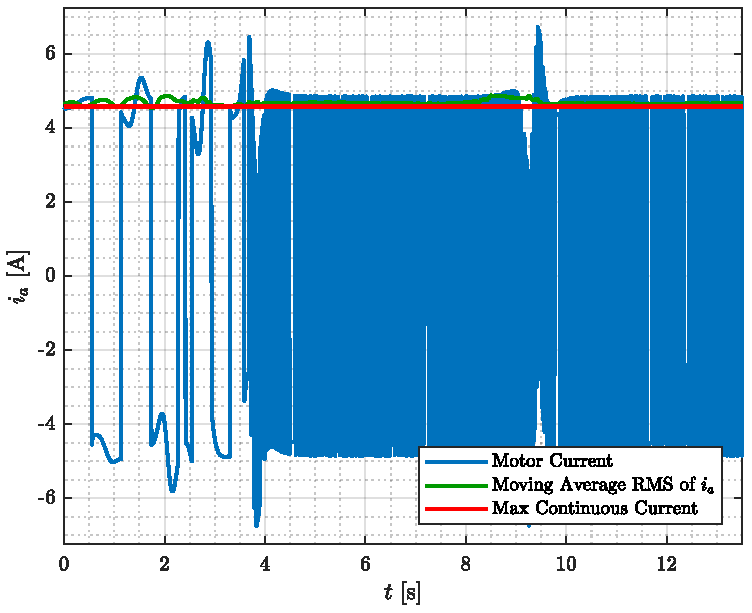
\includegraphics[width=.52\textwidth]{figures/ia_2_noConX}
  \caption{The sign-function in the control law causes excessive switching in the output, thus, the design is not feasible for a real system implementation.}
  \label{fig:ia_2_noConX}
\end{figure}
%
This actuation behavior is not feasible in a real system and attempted implementation will cause chattering resulting in unwanted behavior and wear of the motor. In next section it is attempted to solve this issue, while keeping some of the performance of this approach.
%
%\begin{figure}[H]
%  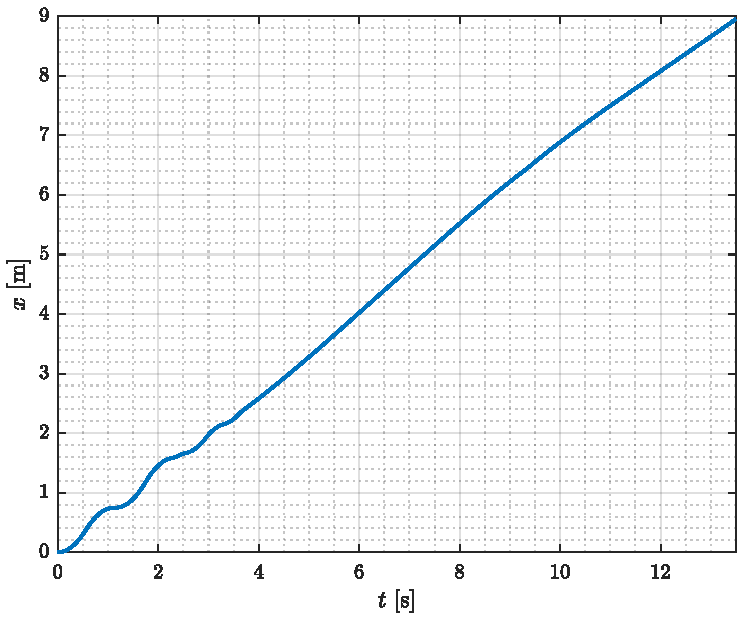
\includegraphics[width=.6\textwidth]{figures/x_2_noConX}
%  \caption{x2noConX}
%  \label{fig:x_2_noConX}
%\end{figure}
%\begin{figure}[H]
%  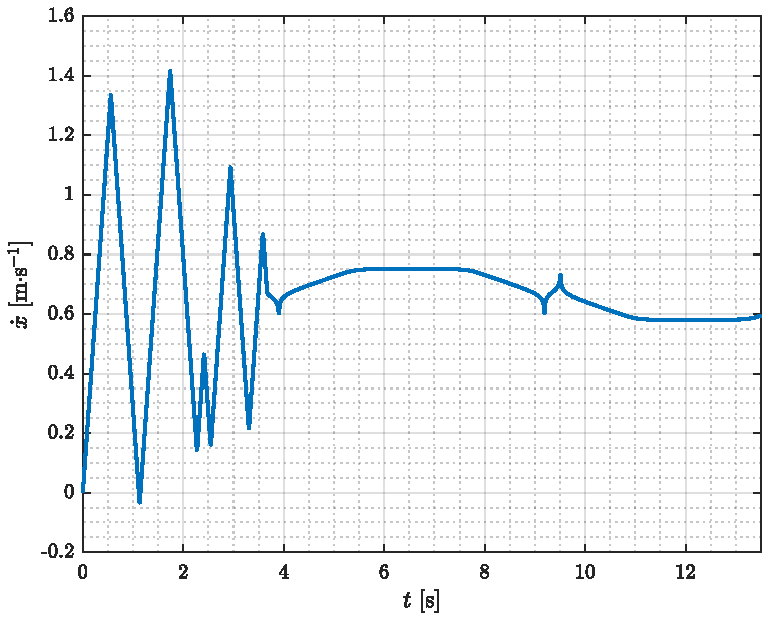
\includegraphics[width=.6\textwidth]{figures/xDot_2_noConX}
%  \caption{xDot2noConX}
%  \label{fig:xDot_2_noConX}
%\end{figure}
%\begin{figure}[H]
%  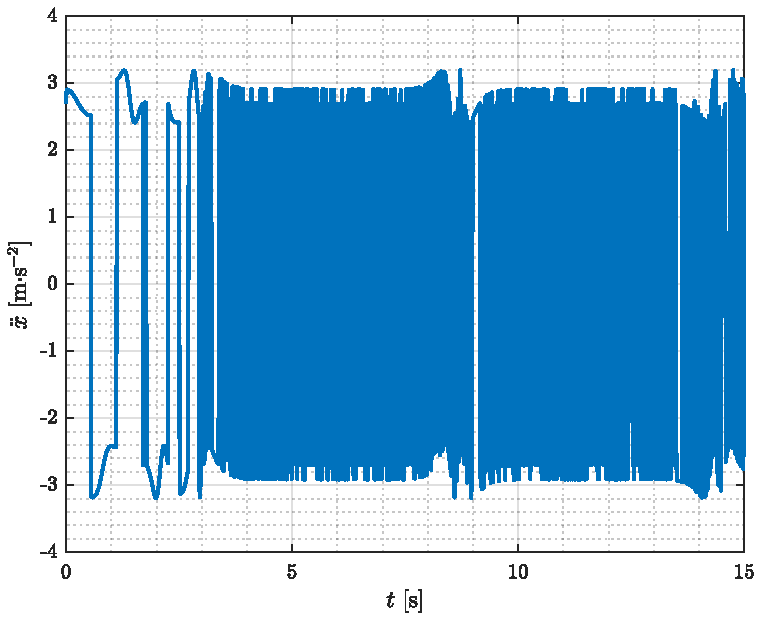
\includegraphics[width=.6\textwidth]{figures/xDotDot_2_noConX}
%  \caption{xDotDot2noConX}
%  \label{fig:xDotDot_2_noConX}
%\end{figure}
%\begin{figure}[H]
%  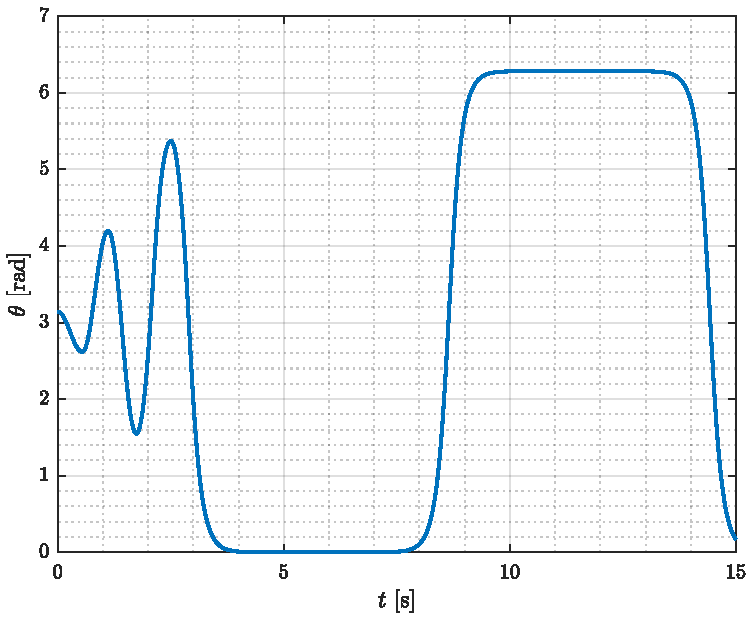
\includegraphics[width=.6\textwidth]{figures/theta_2_noConX}
%  \caption{theta2noConX}
%  \label{fig:theta_2_noConX}
%\end{figure}
%\begin{figure}[H]
%  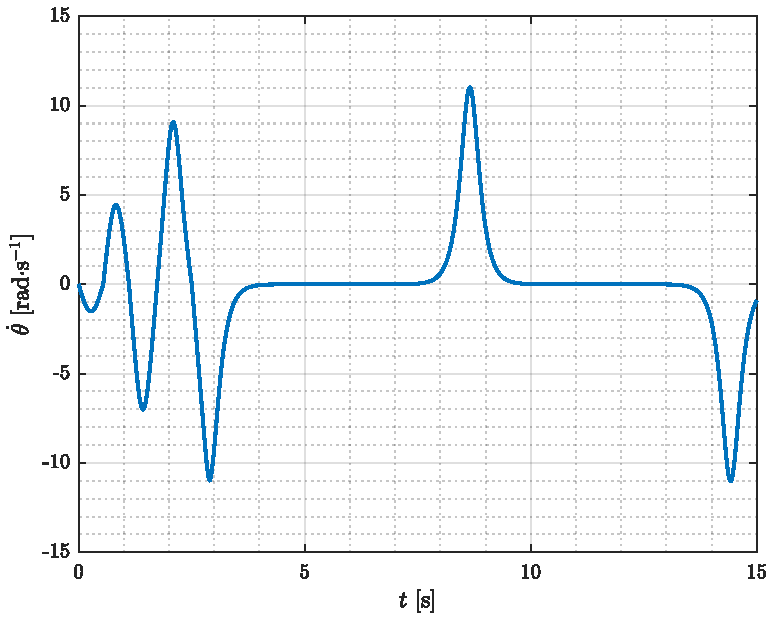
\includegraphics[width=.6\textwidth]{figures/thetaDot_2_noConX}
%  \caption{thetaDot2noConX}
%  \label{fig:thetaDot_2_noConX}
%\end{figure}
%\begin{figure}[H]
%  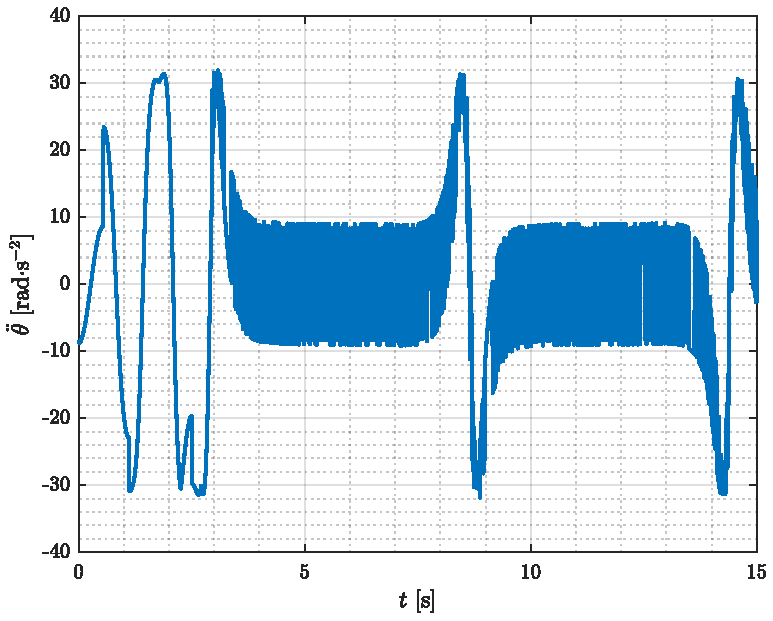
\includegraphics[width=.6\textwidth]{figures/thetaDotDot_2_noConX}
%  \caption{thetaDotDot2noConX}
%  \label{fig:thetaDotDot_2_noConX}
%\end{figure}
%
%
%

%------------------------------------------------------------------------------------------
%-------------------My Sat-based solution--------------------------------------------------
%------------------------------------------------------------------------------------------

%It is possible to implement a less aggressive version of this idea by using a saturation function to approximate the sign function around zero,
%\begin{align}
%  a_c &= k\ \mathrm{sat}(-\tfrac{1}{\varepsilon}E_\Delta \cos \theta \dot{\theta})  \ \ \ ,   \label{eq:accControlLaw2_2} 
%\end{align}
%where $\varepsilon$ decides the slope of the saturation function around zero,
%\begin{align}
%  \text{sat}\left( \frac{f}{\varepsilon} \right) &=
%  \begin{cases}
%    \ \ \frac{f}{\varepsilon}                             &, \ \ \ \ \mathrm{if} \ | \frac{f}{\varepsilon} |  < 1 \\
%    \ \ \mathrm{sgn}\left( \frac{f}{\varepsilon} \right)  &, \ \ \ \ \mathrm{if} \ | \frac{f}{\varepsilon} |  > 1 \\
%    \ \ 1                                                 &, \ \ \ \ \mathrm{if} \ \cos \theta \dot{\theta} = 0 \ \ \ ,
%  \end{cases}
%  \label{eq:satuationFunction1}
%\end{align}
%where $f$ is some input to the sat-function.
%In the simulation $k = 2.7$ as before and $\varepsilon = 0.01$ to avoid excessive switching while maintaining a relatively close approximation of the sign-function.\\
%This control strategy achieves the energy reference in about three seconds, \autoref{fig:Edelta_3_noConX}, as is the case of the sign strategy, \autoref{fig:Edelta_2_noConX}. Further, from \autoref{fig:phase_3_noConX}, the system still reaches a near perfect heteroclinic orbit.
%%
%\begin{figure}[H]
%  \hspace{-10pt}
%  \captionbox
%  {
%    The approximation of the sign approach using a saturation function shows no loss in performance when comparing the energy error.
%    \label{fig:Edelta_3_noConX}
%  }
%  {
%    \hspace{-1cm}
%    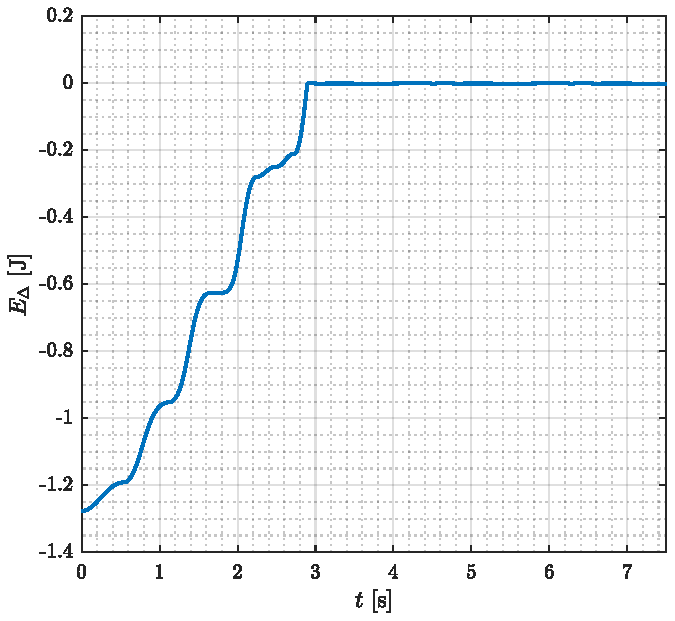
\includegraphics[width=.448\textwidth]{figures/Edelta_3_noConX}
%  }
%  \hspace{20pt}
%  \captionbox 
%  {
%    The heteroclinic orbit is still reached, however, with a more realistic trajectory at the approach of the equilibrium points.
%    \label{fig:phase_3_noConX}
%  }
%  {
%    \hspace{-1cm}
%    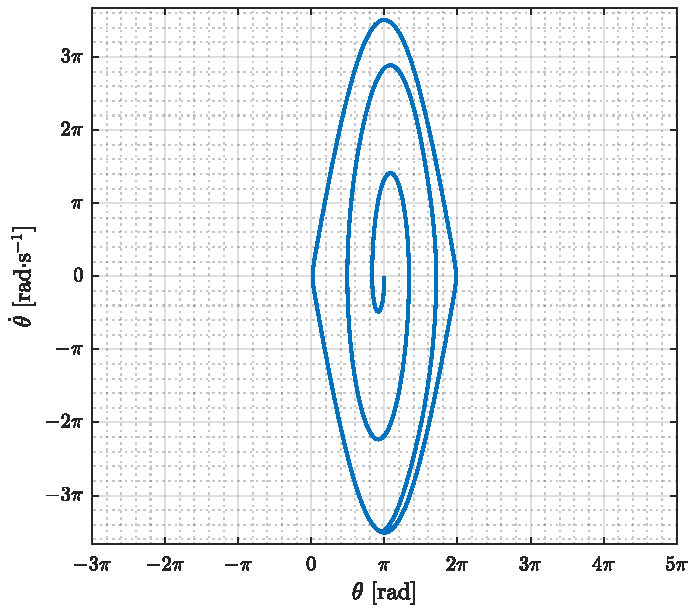
\includegraphics[width=.46\textwidth]{figures/phase_3_noConX}
%  }  
%\end{figure}
%%
%The cart still drifts as expected, see \autoref{fig:ani_3_noConX}, and the equilibrium points are maintained for shorter durations, which is expected with less control switching.
%%
%\begin{figure}[H]
%  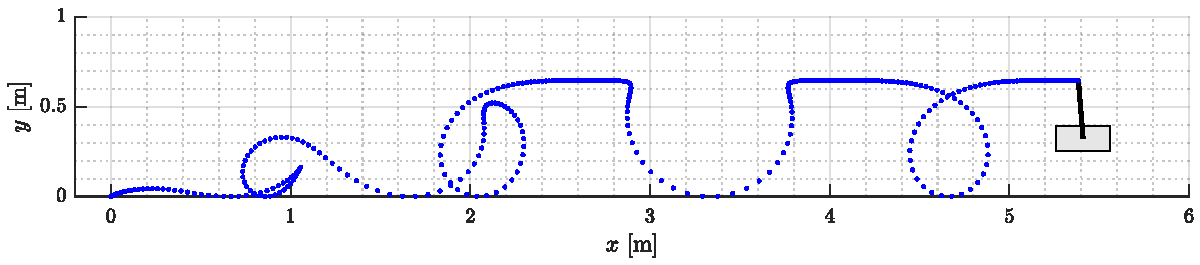
\includegraphics[width=.7\textwidth]{figures/ani_3_noConX}
%  \caption{This strategy performs well. The drifting problem is solved later.}
%  \label{fig:ani_3_noConX}
%\end{figure}
%%
%The excessive switching on the control output is successfully avoided, see \autoref{fig:ia_3_noConX}, resulting in a much more realistic control signal compared to that in \autoref{fig:ia_2_noConX}.
%%
%\begin{figure}[H]
%  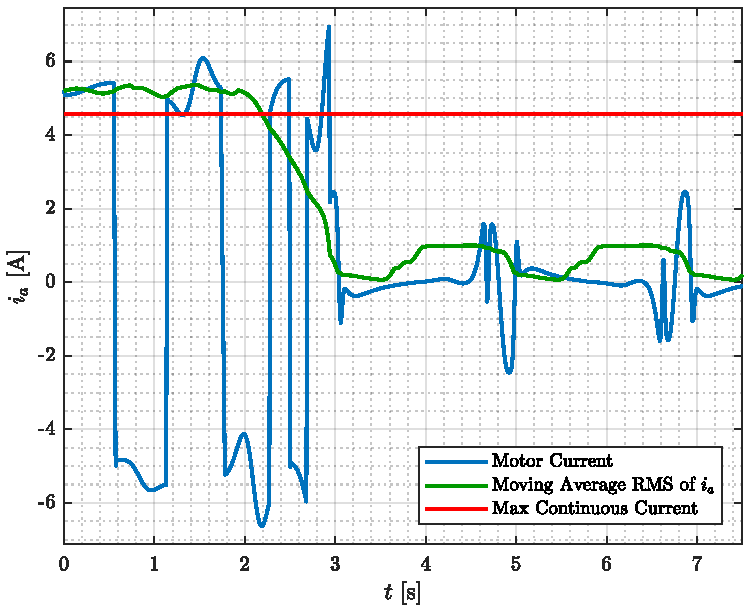
\includegraphics[width=.52\textwidth]{figures/ia_3_noConX}
%  \caption{The control signal using the saturation approximation of the sign-function is much more realistic for implementation.}
%  \label{fig:ia_3_noConX}
%\end{figure}
%The next section explores an other approach based on the same general idea and motivation.

%------------------------------------------------------------------------------------------
%------------------------------------------------------------------------------------------
%------------------------------------------------------------------------------------------
%
%
%\begin{figure}[H]
%  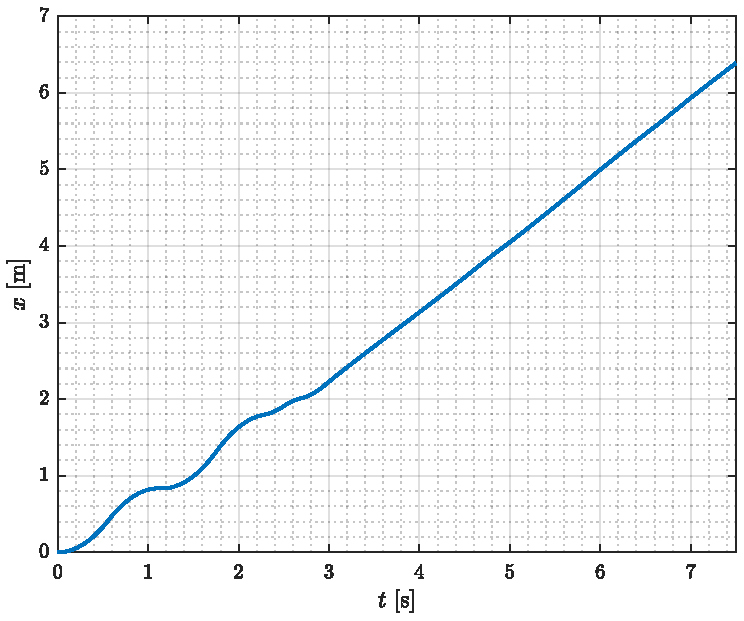
\includegraphics[width=.6\textwidth]{figures/x_3_noConX}
%  \caption{x3noConX}
%  \label{fig:x_3_noConX}
%\end{figure}
%\begin{figure}[H]
%  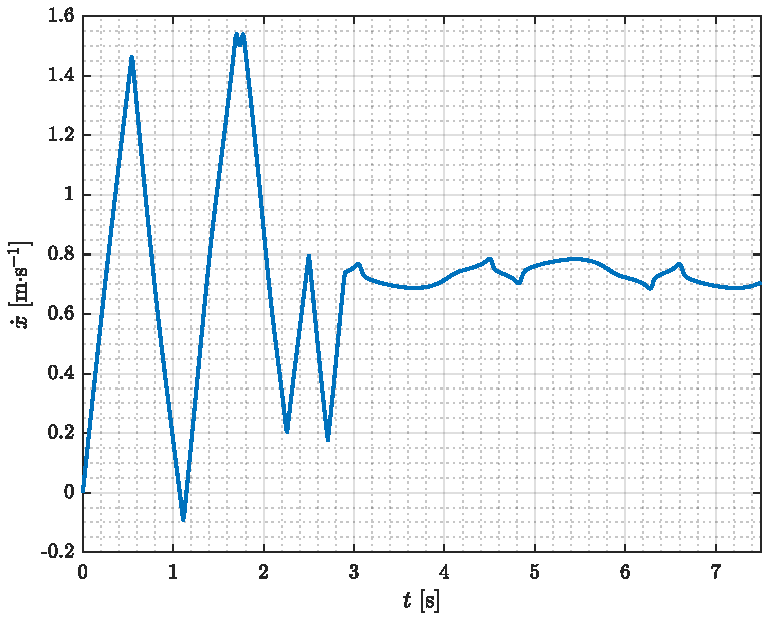
\includegraphics[width=.6\textwidth]{figures/xDot_3_noConX}
%  \caption{xDot3noConX}
%  \label{fig:xDot_3_noConX}
%\end{figure}
%\begin{figure}[H]
%  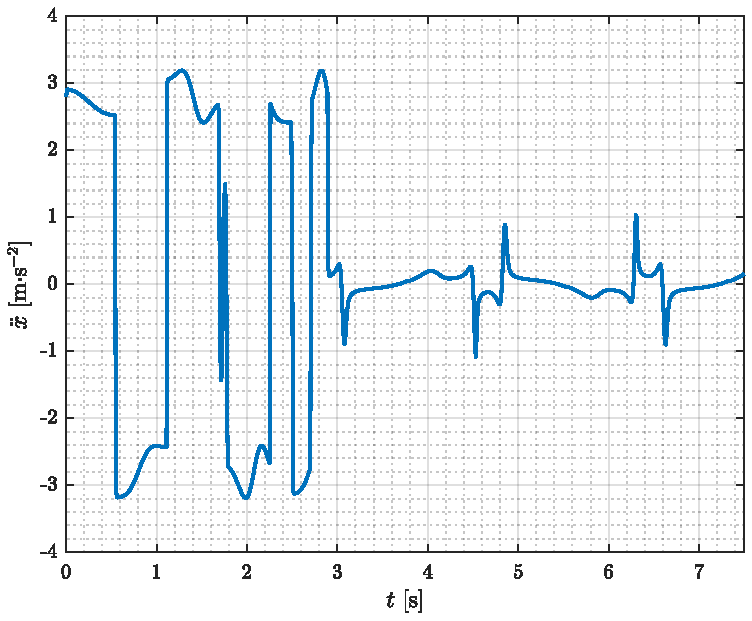
\includegraphics[width=.6\textwidth]{figures/xDotDot_3_noConX}
%  \caption{xDotDot3noConX}
%  \label{fig:xDotDot_3_noConX}
%\end{figure}
%\begin{figure}[H]
%  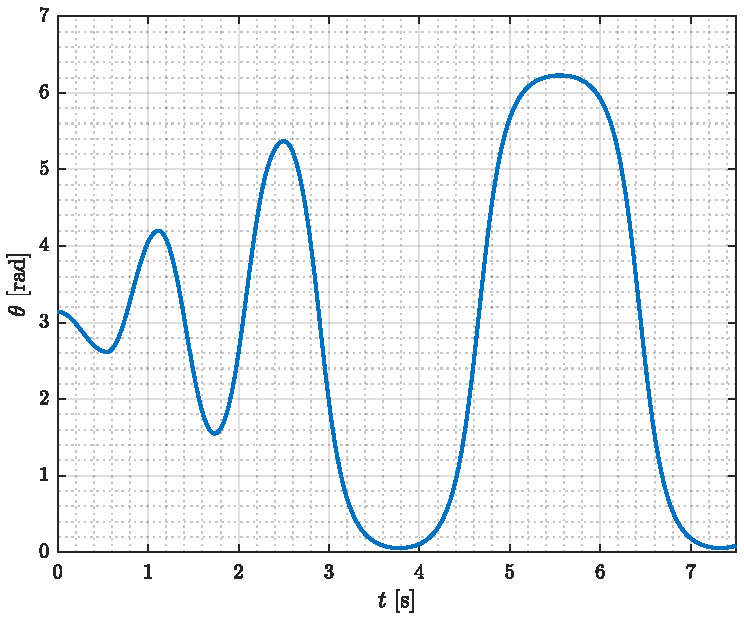
\includegraphics[width=.6\textwidth]{figures/theta_3_noConX}
%  \caption{theta3noConX}
%  \label{fig:theta_3_noConX}
%\end{figure}
%\begin{figure}[H]
%  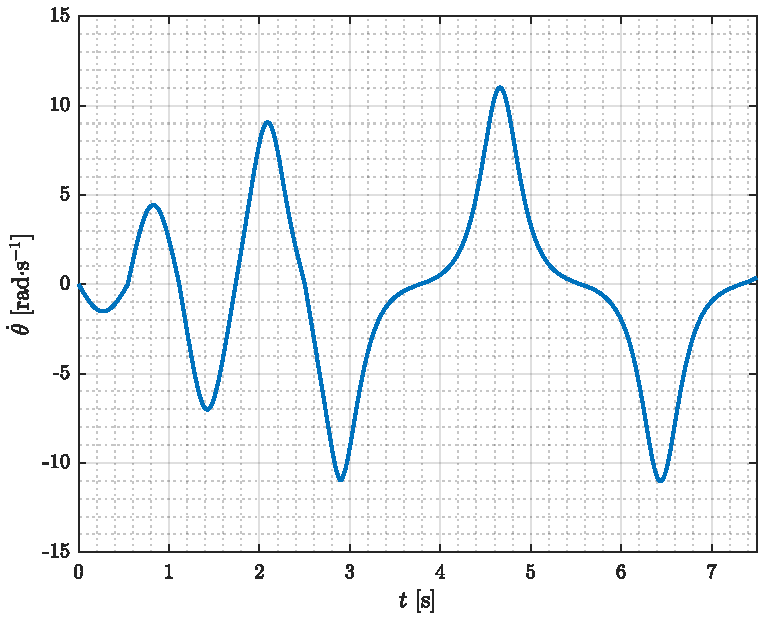
\includegraphics[width=.6\textwidth]{figures/thetaDot_3_noConX}
%  \caption{thetaDot3noConX}
%  \label{fig:thetaDot_3_noConX}
%\end{figure}
%\begin{figure}[H]
%  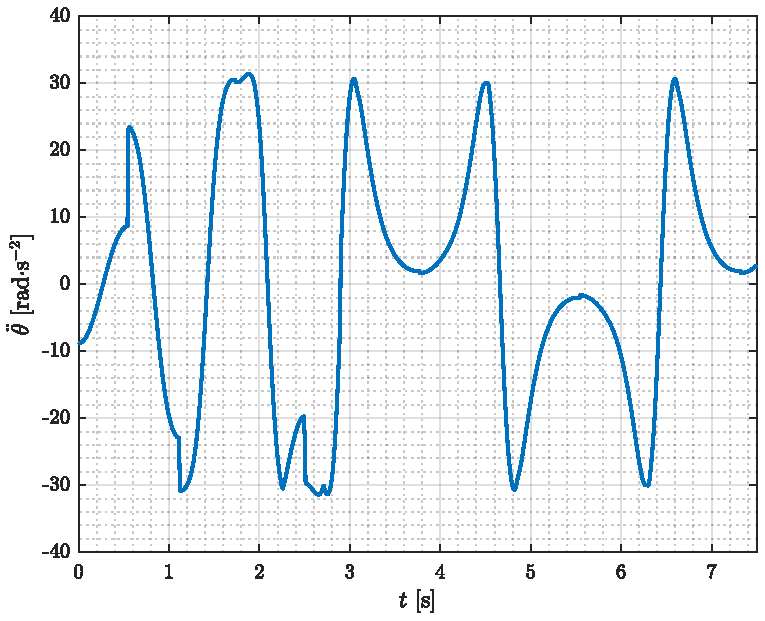
\includegraphics[width=.6\textwidth]{figures/thetaDotDot_3_noConX}
%  \caption{thetaDotDot3noConX}
%  \label{fig:thetaDotDot_3_noConX}
%\end{figure}

\section{Sat-Based Energy Control}
To avoid the excessive switching of the sign-based controller a different strategy using a saturation function is investigated,
\begin{align}
  a_c &= \mathrm{sat}(-k E_\Delta \mathrm{sgn}(\cos \theta \dot{\theta}))  \ \ \ ,   \label{eq:accControlLaw3} 
\end{align}
where 
\begin{align}
\mathrm{sgn}( s ) &=
\begin{cases}
\ \ \phantom{-}1 & \ \  | s |  \geq 0 \\
\ \           -1 & \ \  | s |  <    0 \ \ \ ,
\end{cases}
\label{eq:sgnFunction1}
\end{align}
and the sat-function saturates at the minimum/maximum allowed acceleration. The known limitation is $i_{max} = 4.58$ as stated in \autoref{table:systemParameters}, from which the maximum control, $u$, can be calculated,
\begin{align}
  u_{max} &=  \frac{k_{\tau}}{r} \ \ \ ,    \label{eq:maxU} 
\end{align}
and finally, by disregarding the pendulum behavior and cart friction from the dynamics in \autoref{eq:energyDerivedDynamicEquation1},
\begin{align}
  a_{max} &= \frac{u_{max}}{M+m} \ \ \ .   \label{eq:maxAcc} 
\end{align}
As this is a crude estimate \SI{0.1}{m\cdot s^{-2}} is subtracted from the estimated $a_{max}$ in following simulations to stay within the actuation limits. The saturation function is then,
\begin{align}
  \text{sat}(s) &=
  \begin{cases}
    \ \ s                           & \ \  | s |  \leq a_{max} \\
    \ \ \mathrm{sgn}( s )\ a_{max}  & \ \  | s |  >  a_{max} \ \ \ .
  \end{cases}
  \label{eq:satuationFunction}
\end{align}
Notice how the sgn-function in this control law, \autoref{eq:accControlLaw3}, only takes $\cos \theta \dot{\theta}$ as input. Contrary to the sign-based controller which also included $E_\Delta$ causing the need for complicated restrictions in the definition of the sgn-function.

Choice of $k$ decides how aggressive the controller should be. Larger values of $k$ drives the control into saturation faster thus actuating more like the sign-based controller in \autoref{eq:accControlLaw2}. At lower values of $k$ the operation will not reach saturation as fast thus behaving more like the first energy based controller in \autoref{eq:accControlLaw}. For an effective swing up behavior $k=200$ is chosen, thus approaching the behavior of the sign-based controller, which makes sense as this is the theoretically ideal solution.\\
This control strategy achieves the energy reference in about three seconds, \autoref{fig:Edelta_4_noConX}, as is the case of the sign-based strategy, \autoref{fig:Edelta_2_noConX}. Further, from  \autoref{fig:phase_4_noConX}, the system still reaches a near perfect heteroclinic orbit.
%
\begin{figure}[H]
  \hspace{-10pt}
  \captionbox
  {
    The sat-based controller shows no loss in performance when comparing the energy error to that of the sign-based approach.
    \label{fig:Edelta_4_noConX}
  }
  {
    \hspace{-1cm}
    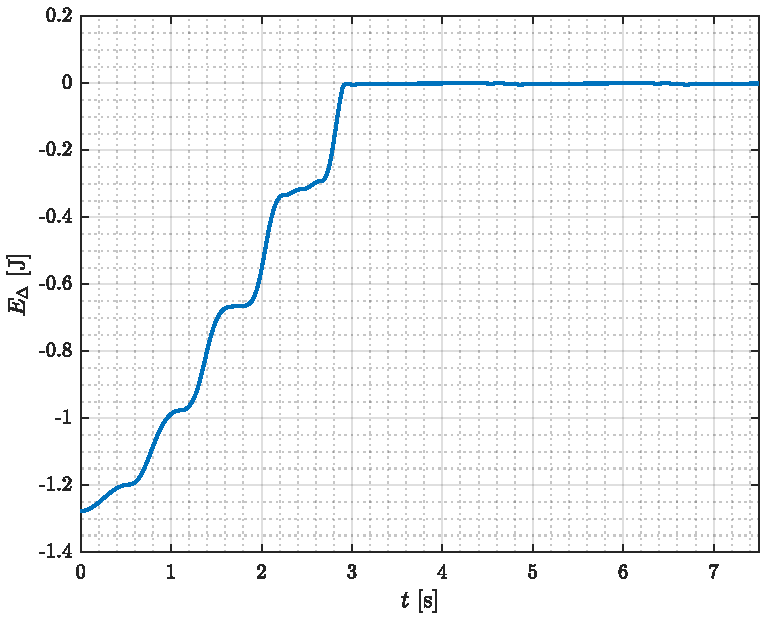
\includegraphics[width=.448\textwidth]{figures/Edelta_4_noConX}
  }
  \hspace{20pt}
  \captionbox 
  {
    The heteroclinic orbit is still reached, however, with a more realistic trajectory at the approach of the equilibrium points.
    \label{fig:phase_4_noConX}
  }
  {
    \hspace{-1cm}
    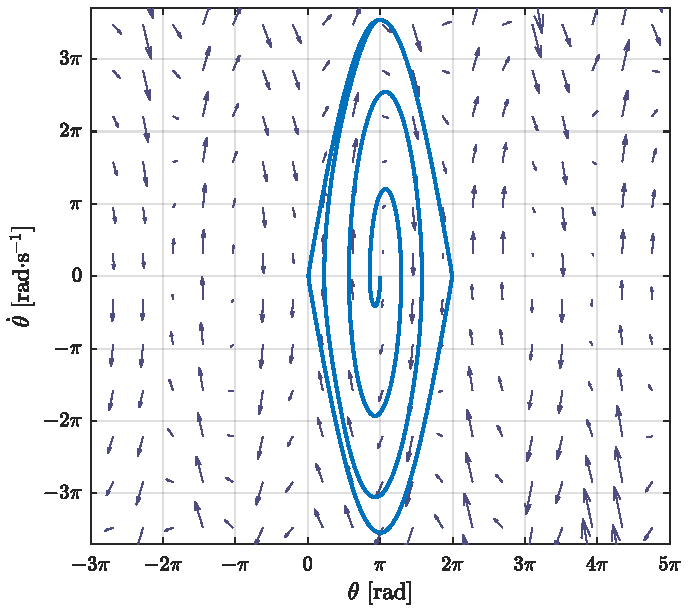
\includegraphics[width=.46\textwidth]{figures/phase_4_noConX}
  }  
\end{figure}
%
The cart still drifts as expected, see \autoref{fig:ani_4_noConX}, and the equilibrium points are maintained for shorter duration, which is expected with less control switching.
%
\autoref{fig:ani_4_noConX}.
\begin{figure}[H]
  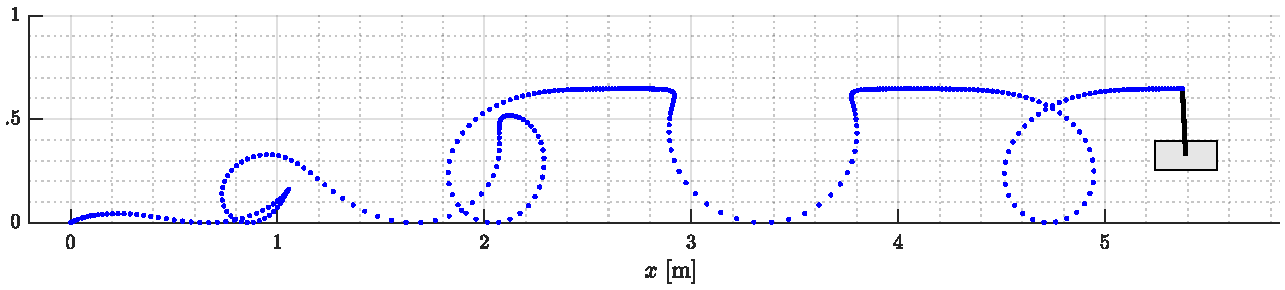
\includegraphics[width=.7\textwidth]{figures/ani_4_noConX}
  \caption{This strategy performs well. The drifting problem is solved later.}
  \label{fig:ani_4_noConX}
\end{figure}
%
The excessive switching on the control output is successfully avoided, see \autoref{fig:ia_4_noConX}, resulting in a much more realistic control signal compared to that in \autoref{fig:ia_2_noConX}.
%
\begin{figure}[H]
  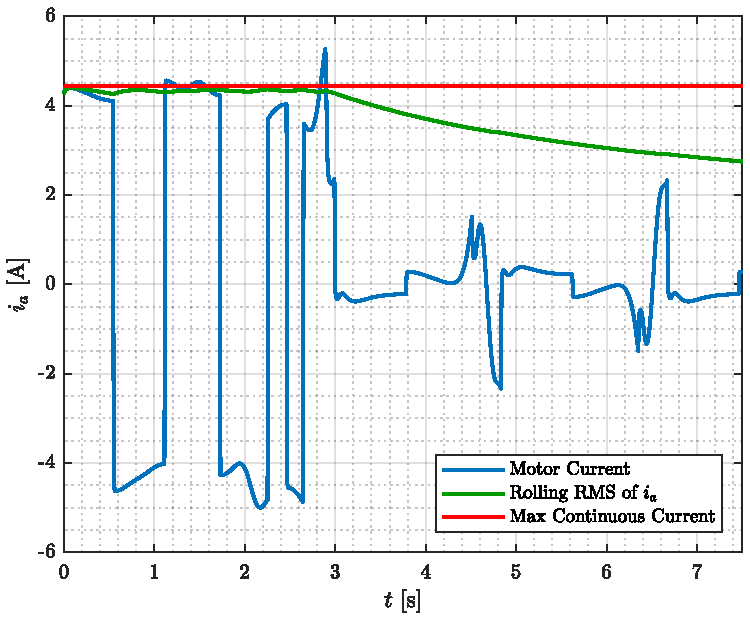
\includegraphics[width=.52\textwidth]{figures/ia_4_noConX}
  \caption{The control signal using the sat-based approach is much more realistic for implementation as the excessive switching of the sign-based controller is successfully avoided.}
  \label{fig:ia_4_noConX}
\end{figure}
%
The design of the energy based control law, \autoref{eq:accControlLaw3}, is concluded. The problem of controlling the cart position still remains. In the following, the performance of this control law is subjected to the disturbance caused by added control on the cart position and velocity.
%
%
%\begin{figure}[H]
%  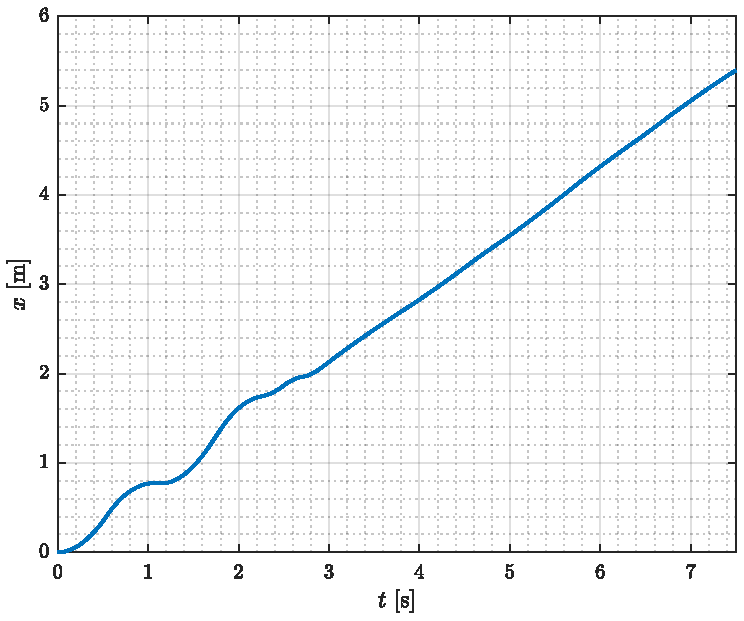
\includegraphics[width=.6\textwidth]{figures/x_4_noConX}
%  \caption{x4noConX}
%  \label{fig:x_4_noConX}
%\end{figure}
%\begin{figure}[H]
%  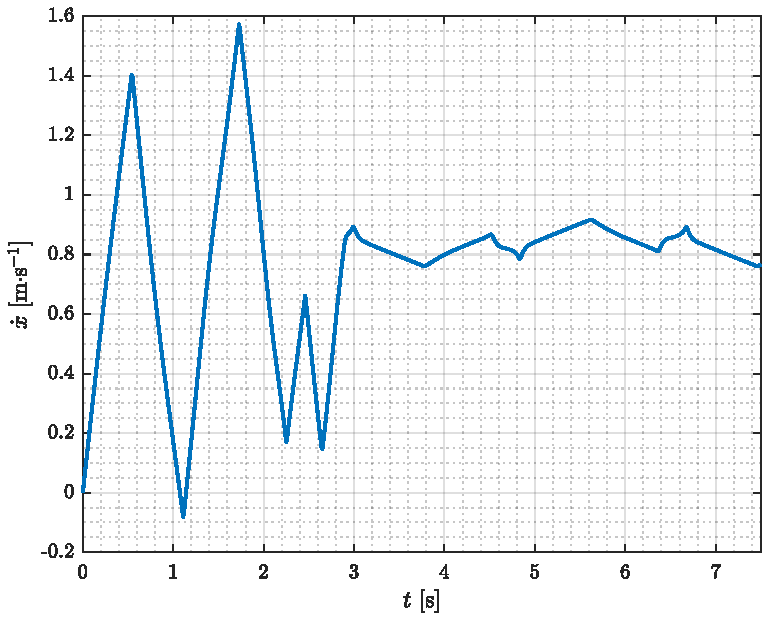
\includegraphics[width=.6\textwidth]{figures/xDot_4_noConX}
%  \caption{xDot4noConX}
%  \label{fig:xDot_4_noConX}
%\end{figure}
%\begin{figure}[H]
%  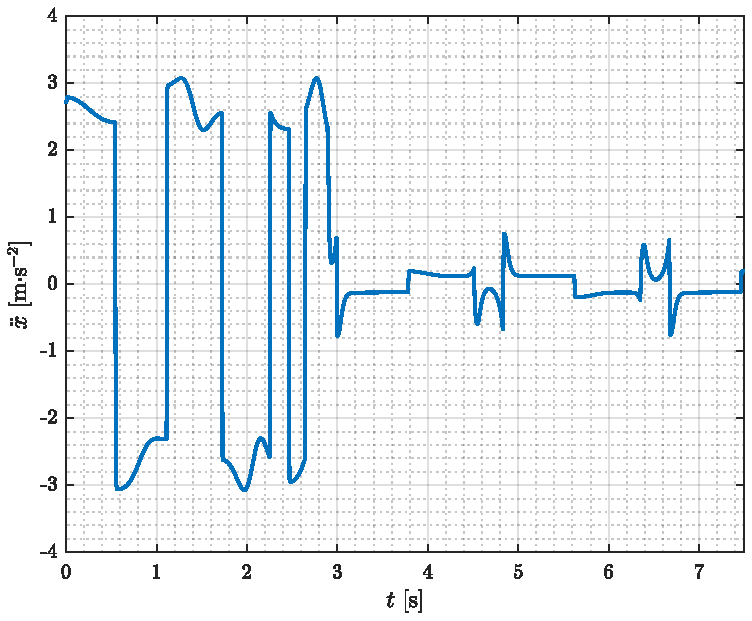
\includegraphics[width=.6\textwidth]{figures/xDotDot_4_noConX}
%  \caption{xDotDot4noConX}
%  \label{fig:xDotDot_4_noConX}
%\end{figure}
%\begin{figure}[H]
%  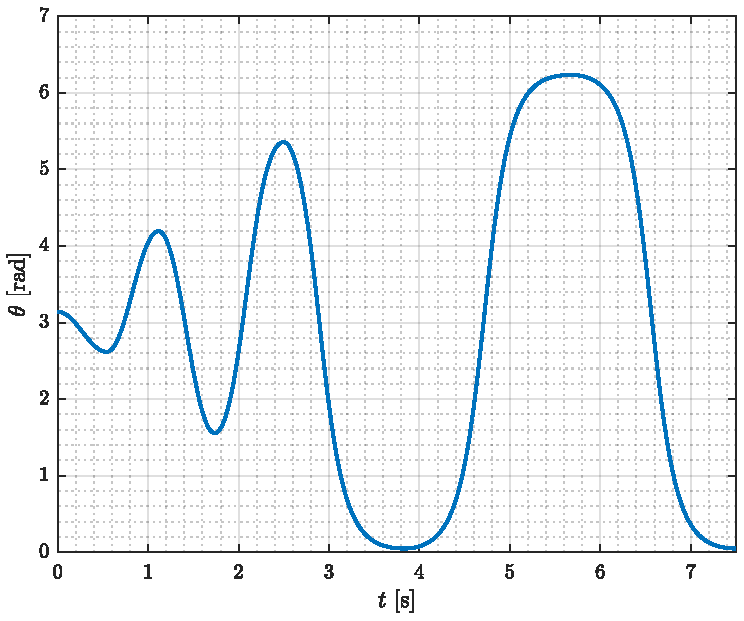
\includegraphics[width=.6\textwidth]{figures/theta_4_noConX}
%  \caption{theta4noConX}
%  \label{fig:theta_4_noConX}
%\end{figure}
%\begin{figure}[H]
%  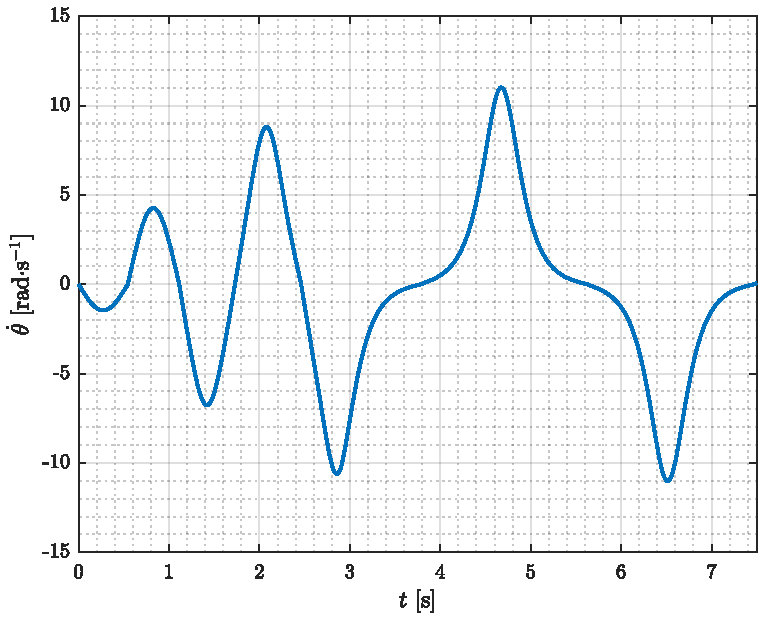
\includegraphics[width=.6\textwidth]{figures/thetaDot_4_noConX}
%  \caption{thetaDot4noConX}
%  \label{fig:thetaDot_4_noConX}
%\end{figure}
%\begin{figure}[H]
%  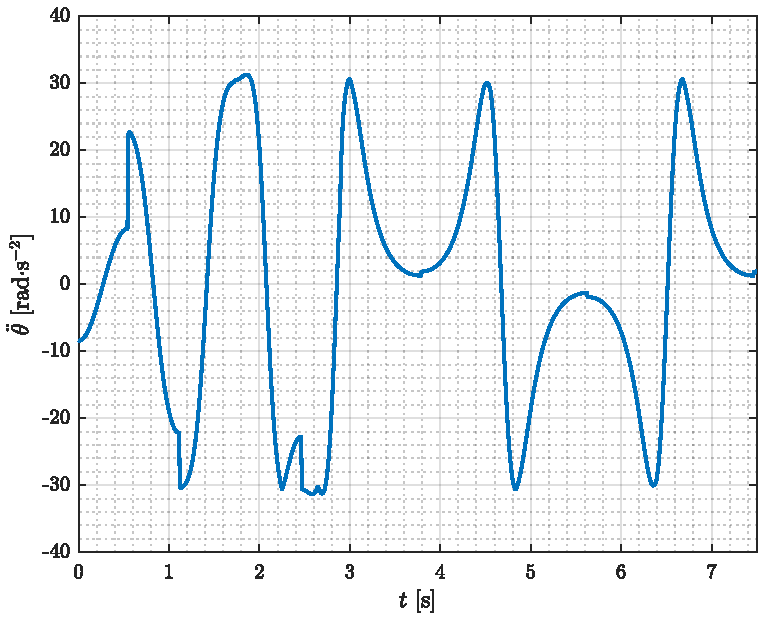
\includegraphics[width=.6\textwidth]{figures/thetaDotDot_4_noConX}
%  \caption{thetaDotDot4noConX}
%  \label{fig:thetaDotDot_4_noConX}
%\end{figure}

\section{Cart Position and Velocity Control}
To solve the cart drifting problem along $x$ a linear controller is designed and added to the control law,
\begin{align}
  a_c &= \psi(x_1,x_3) + v(x_2,x_4) \ \ \ ,   \label{eq:combiControl} 
\end{align}
where $\psi(x_1,x_3)$ is the energy controller and $v(x_2,x_4)$ is the linear controller. While these two controllers depend on different states, they still influence and act as unmodeled disturbances to one another. The position and velocity control, $v(x_2,x_4)$, adds and subtracts energy, therefore could cause the energy controller, $\psi(x_1,x_3)$, to overshoot. One solution to this potential problem could be to slightly lower the energy reference. However, swing-up is often designed with a higher energy reference such that the catch controller has some entry velocity at the unstable equilibrium.\\
With these considerations in mind, the design of $v(x_2,x_4)$ is proceeded. Considering the cart without friction and assuming any influence of the pendulum dynamics and the energy control to be unmodeled disturbances of the system. This reduces the model to the mechanical drawing seen in \autoref{fig:mechanicalDrawingSimple}.
%
\begin{figure}[H]
  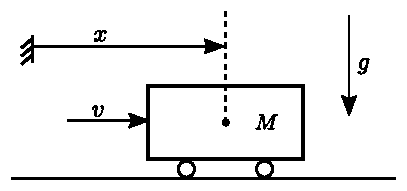
\includegraphics[width=.35\textwidth]{figures/mechanicalDrawingSimple}
  \caption{Mechanical drawing of the reduced model used for position control.}
  \label{fig:mechanicalDrawingSimple}
\end{figure}
%
The dynamics are then,
\begin{align}
  M \ddot{x} &=  v \ \ \ ,  \label{eq:simpleDynamics} 
\end{align}
and selecting new states $ [\ z_1\ \ z_2\ ]^\mathrm{T} = [\ x\ \ \dot{x}\ ]^\mathrm{T} $, the linear state space is,\vspace{6pt}
\begin{align}
  \begin{bmatrix}
    \dot{z_1} \\
    \dot{z_2}
  \end{bmatrix}
  &=
  \underbrace{
    \begin{bmatrix}
      0 & 1 \\
      0 & 0
    \end{bmatrix}
  }_{A}
  \begin{bmatrix}
    z_1 \\
    z_2
  \end{bmatrix}
  +
  \underbrace{
    \begin{bmatrix}
      0 \\
      \tfrac{1}{M}
    \end{bmatrix}
  }_{B}
  v
  \label{eq:simpleLinearStateSpace} \ \ \ .
\end{align}
%
The closed loop poles are placed in $p = [\ -1\ -2 \ ] $ using matlab \textit{place()}-command to obtain linear feedback gains, $\vec{k_1} = [\ 10.5460\ \ 15.8190\ ]$, resulting in the controller,
\begin{align}
  v &= -\vec{k_1} \vec{z} \ \ \ ,  \label{eq:linearFeedbackSimple} 
\end{align}
where $\vec{z} = [\ x\ \ \dot{x}\ ]^\mathrm{T}$, such that,
\begin{align}
  v(x_2,x_4) &= -\vec{k_1}  [\ x_2\ \ x_4\ ]^\mathrm{T} \ \ \ ,    \label{eq:linearFeedbackSimple2} 
\end{align}
in therms of the full system. This control is added to the sat-based design and simulations are run without changing any previously designed gains.

\autoref{fig:Edelta_4_conX} shows the energy error reaching zero, taking one second longer under the influence of the linear controller, compared to \autoref{fig:Edelta_4_noConX}.
%
\begin{figure}[H]
  \hspace{-10pt}
  \captionbox 
  {
    The sat-based controller reaches the reference in about four seconds, compared to three seconds it took without position and velocity control.
    \label{fig:Edelta_4_conX}
  }
  {
    \hspace{-1cm}
    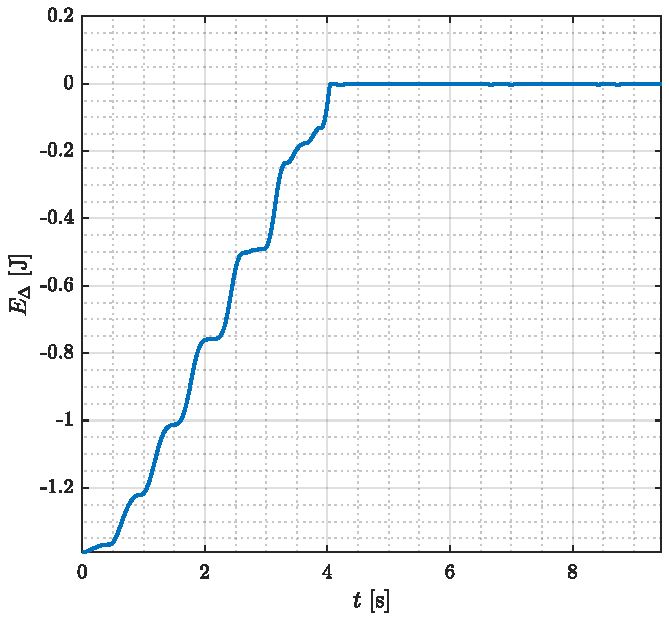
\includegraphics[width=.448\textwidth]{figures/Edelta_4_conX}
  }
  \hspace{20pt}
  \captionbox 
  {
    Though the sat-based energy controller reaches its reference one second slower when kept around $x = 0$, it still reaches the heteroclinic orbit with no overshoot.
    \label{fig:phase_4_conX}
  }
  {
    \hspace{-1cm}
    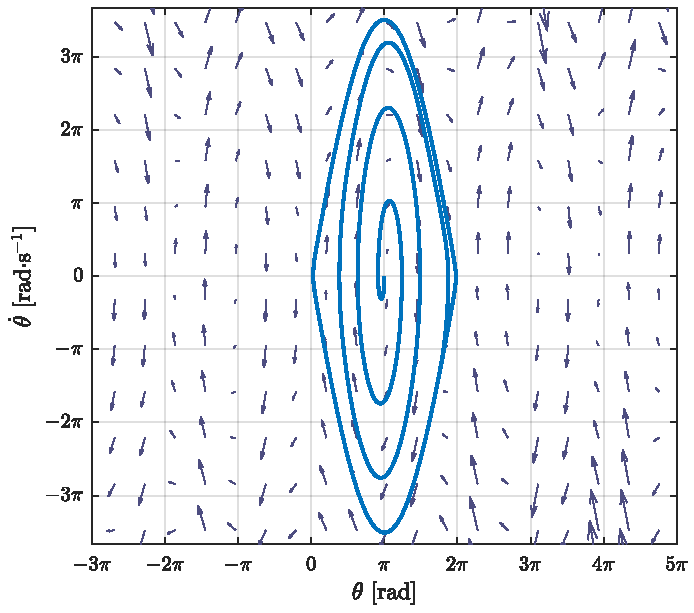
\includegraphics[width=.46\textwidth]{figures/phase_4_conX}
  }
\end{figure}
%
In the phase portrait, see \autoref{fig:phase_4_conX}, it is clear that the sat-based controller still reaches the heteroclinic orbit.
\autoref{fig:ani_4_conX} shows how the linear control of the cart position and velocity successfully keeps the system within the available operating region of the real system.
%
\begin{figure}[H]
  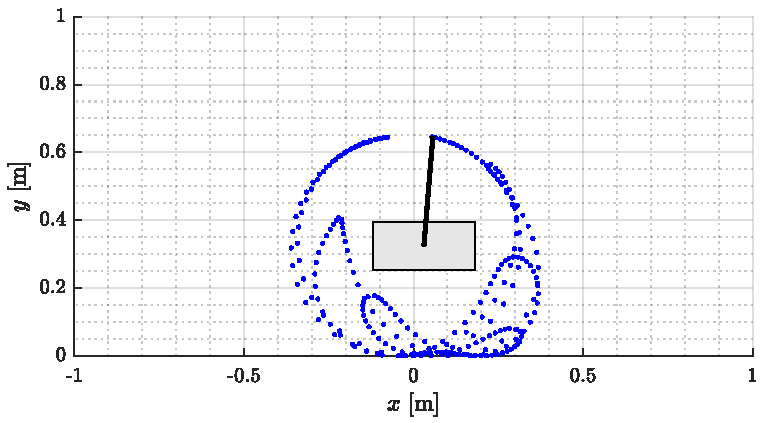
\includegraphics[width=.52\textwidth]{figures/ani_4_conX}
  \caption{The linear control successfully keeps the cart around zero while the energy control approaches the unstable equilibrium.}
  \label{fig:ani_4_conX}
\end{figure}
%
\autoref{fig:ia_4_conX} shows the actuation required, the RMS is lower than it was before the linear controller was added. This could be tuned more tightly, but is left as a margin for now, with the possibility of further tuning during implementation.
%
\begin{figure}[H]
  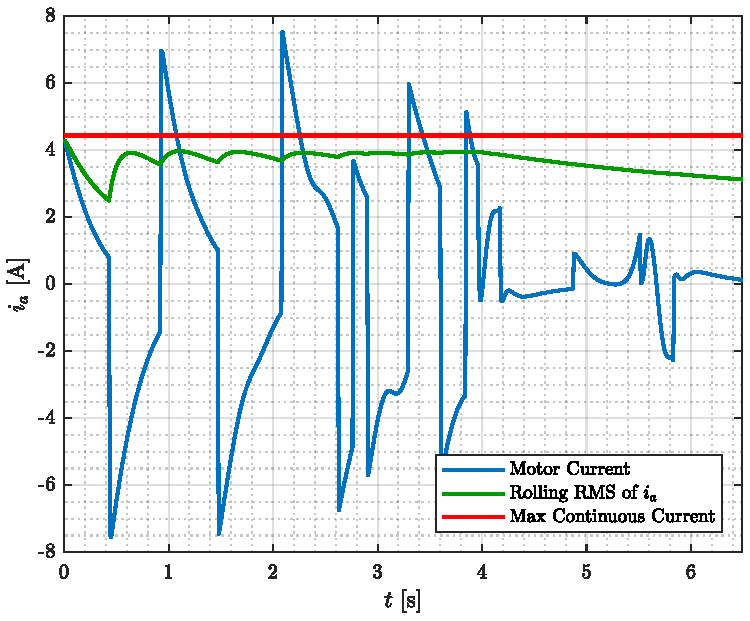
\includegraphics[width=.52\textwidth]{figures/ia_4_conX}
  \caption{The control signal causes less continuous current, as seen by the lower RMS curve, this is left as a margin for now.}
  \label{fig:ia_4_conX}
\end{figure}
%
\autoref{fig:x_4_conX} show the position approaching zero as the energy control settles, which is ideal, as it means the energy controller still has room to operate without fighting the linear feedback controller too much. Similarly, the oscillations around zero are necessary for the energy controller to keep its reference. Further, as seen in \autoref{fig:xDot_4_conX} the velocity of the cart is also eventually controlled to zero by the added liner controller.
\begin{figure}[H]
  \hspace{-10pt}
  \captionbox
  {
    The saturation based controller keeps the cart closer to zero, suggesting less actuation from the energy control.
    \label{fig:x_4_conX}
  }
  {
    \hspace{-1cm}
    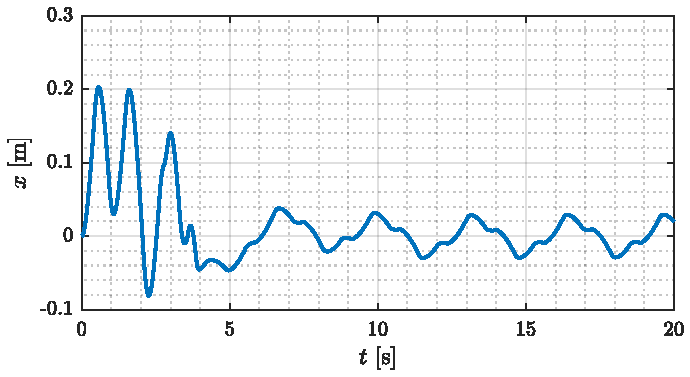
\includegraphics[width=.4\textwidth]{figures/x_4_conX}
  }
  \hspace{20pt}
  \captionbox 
  {
    Zero velocity is obtained quite effectively after the energy reference is reached.
    \label{fig:xDot_4_conX}
  }
  {
    \hspace{-1cm}
    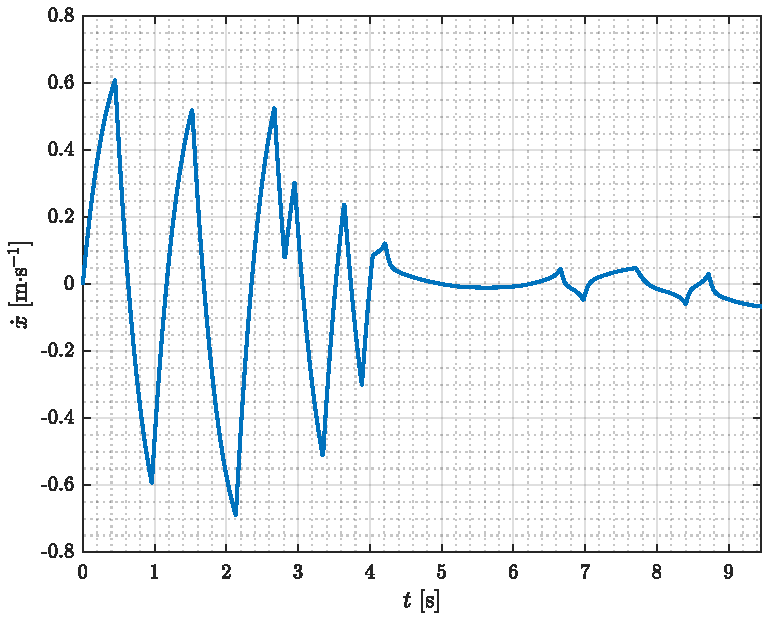
\includegraphics[width=.4\textwidth]{figures/xDot_4_conX}
  }  
\end{figure}
%
These two graphs are simulated over longer time to show that the linear controller reaches its reference.\\
This concludes the design of swing-up control.
%
%
%
%\begin{figure}[H]
%  \includegraphics[width=.6\textwidth]{figures/xDotDot_3_conX}
%  \caption{xDotDot3ConX}
%  \label{fig:xDotDot_3_conX}
%\end{figure}
%\begin{figure}[H]
%  \includegraphics[width=.6\textwidth]{figures/theta_3_conX}
%  \caption{theta3ConX}
%  \label{fig:theta_3_conX}
%\end{figure}
%\begin{figure}[H]
%  \includegraphics[width=.6\textwidth]{figures/thetaDot_3_conX}
%  \caption{thetaDot3ConX}
%  \label{fig:thetaDot_3_conX}
%\end{figure}
%\begin{figure}[H]
%  \includegraphics[width=.6\textwidth]{figures/thetaDotDot_3_conX}
%  \caption{thetaDotDot3ConX}
%  \label{fig:thetaDotDot_3_conX}
%\end{figure}
%
%
%
%\begin{figure}[H]
%  \includegraphics[width=.6\textwidth]{figures/xDotDot_4_conX}
%  \caption{xDotDot4ConX}
%  \label{fig:xDotDot_4_conX}
%\end{figure}
%\begin{figure}[H]
%  \includegraphics[width=.6\textwidth]{figures/theta_4_conX}
%  \caption{theta4ConX}
%  \label{fig:theta_4_conX}
%\end{figure}
%\begin{figure}[H]
%  \includegraphics[width=.6\textwidth]{figures/thetaDot_4_conX}
%  \caption{thetaDot4ConX}
%  \label{fig:thetaDot_4_conX}
%\end{figure}
%\begin{figure}[H]
%  \includegraphics[width=.6\textwidth]{figures/thetaDotDot_4_conX}
%  \caption{thetaDotDot4ConX}
%  \label{fig:thetaDotDot_4_conX}
%\end{figure}